\section{Results}
\label{sec:result}
In this section, we present the results of our study, which are organized as follows: We begin with a description of participant demographics, followed by quantitative and qualitative assessments of cognitive load. We then provide a detailed analysis of participant behaviors. The section concludes with qualitative insights derived from participants' comments on their experiences and the interfaces used. Quantitative data were derived from pen-and-paper surveys and system logs captured during the study. Qualitative insights were generated from interviews conducted after participants completed the survey task. Interview were transcribed and thematically analyzed by the first author. All processed behavioral data are publicly available\footnote{link-to-github} to support transparency and facilitate further research.

\begin{figure}[ht]
    \centering
    % Top figure
    \begin{subfigure}[b]{\textwidth}
        \centering
        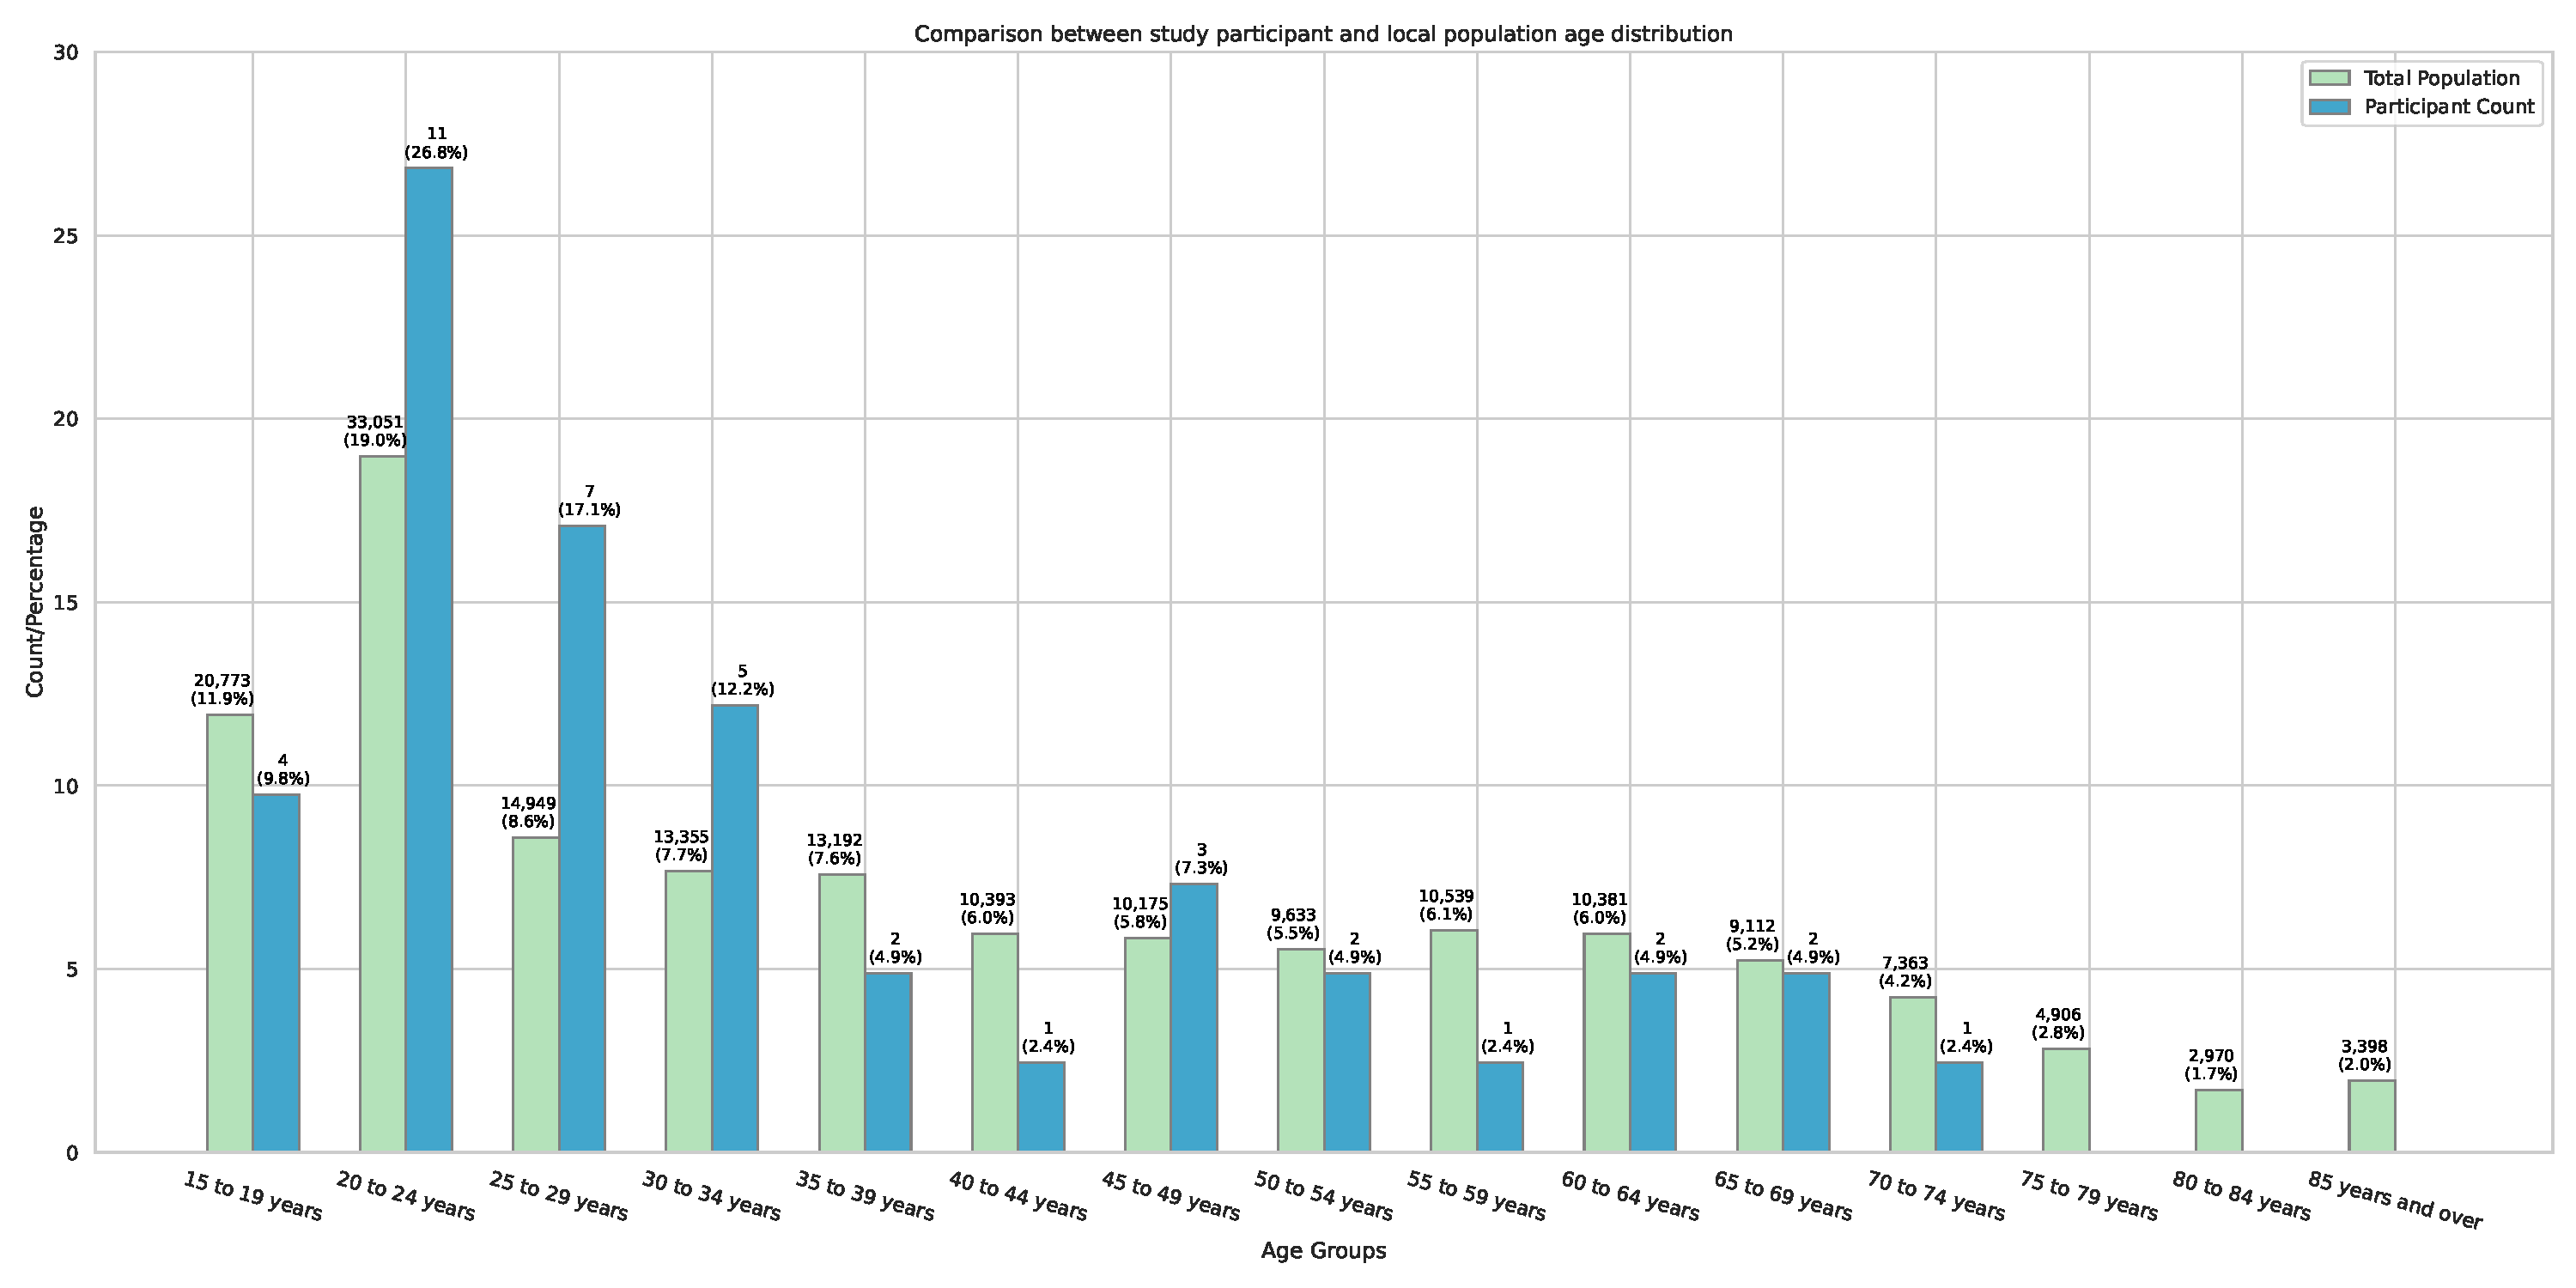
\includegraphics[width=\textwidth]{content/image/demo/demo_age_group_vertical.pdf}
        \caption{Age distribution}
        \label{fig:demoAge}
    \end{subfigure}
    
    \vspace{0.5cm} % Add some vertical space between the rows

    % Bottom figures
    \begin{subfigure}[b]{0.45\textwidth}
        \centering
        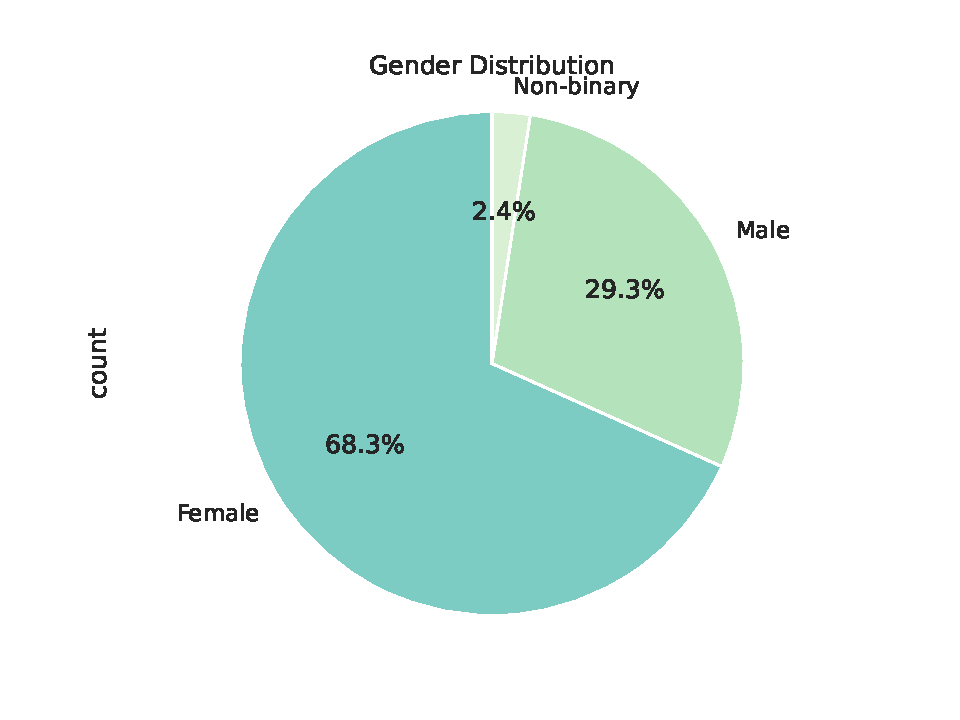
\includegraphics[width=\textwidth]{content/image/demo/demo_gender.pdf}
        \caption{Gender distribution}
        \label{fig:demoGender}
    \end{subfigure}
    \hfill
    \begin{subfigure}[b]{0.45\textwidth}
        \centering
        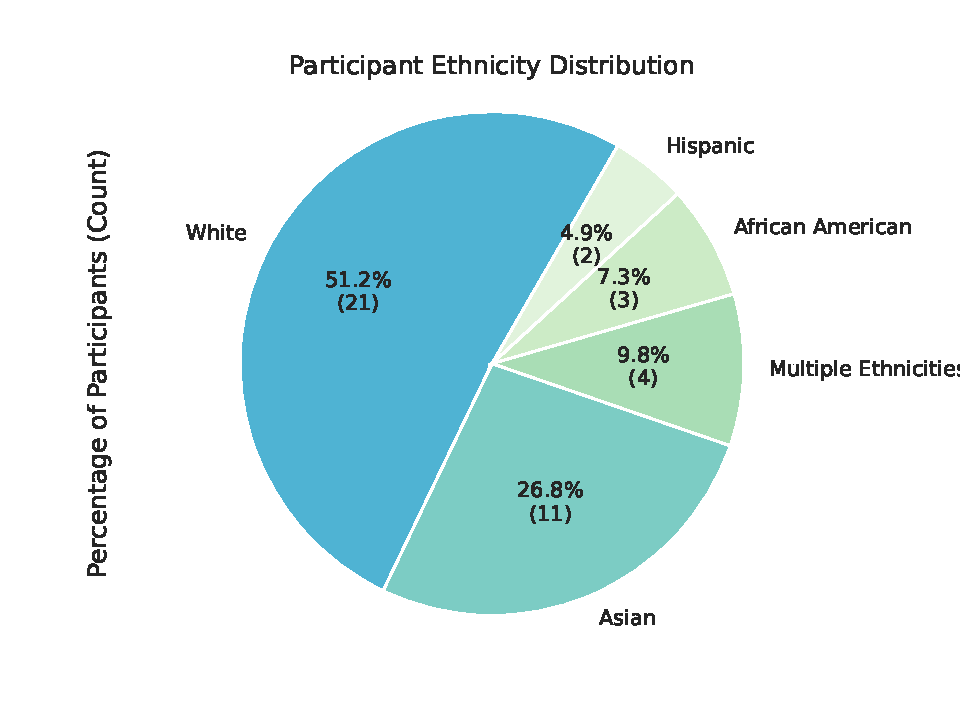
\includegraphics[width=\textwidth]{content/image/demo/demo_ethnicity.pdf}
        \caption{Ethnicity distribution}
        \label{fig:demoEthnicity}
    \end{subfigure}
    
    \caption{Demographic distributions: Age, Gender, and Ethnicity}
    \label{fig:Demographics}
\end{figure}

% maybe more the figure to the appendix?

\subsection{Demographics}
We recruited a total of $41$ participants, allocating ten to each experiment condition. Due to data quality concerns, we excluded one participant's data. The mean age of the participants was $34.63$ years old, with a detailed age distribution presented alongside the county population distribution in Figure~\ref{fig:demoAge}. This comparison reveals that our sample closely matches the county's demographic profile, albeit with a slightly higher representation of younger adults, particularly in the 35-45 age range. As shown in Figure~\ref{fig:demoGender}, the majority of participants skewed toward female.

Regarding ethnicity, $51.2\%$ of the participants identified as White, $26.8\%$ as Asian, $7.3\%$ as African American and $4.9\%$ as Hispanic. Additionally, $9.8\%$ of participants reported mixed ethnicity.

\subsection{Cognitive Load Results}
\label{sec:cog}
In this subsection, we present results in the order of the research questions. We first discuss the distribution of the aggregate NASA-TLX scores across the four experiment conditions, providing interpretation of the results to answer RQ1 and RQ2a. Next, we report the NASA-TLX scores disaggregated into their composite six dimensions to answer RQ2b. Then, we present qualitative and quantitative findings on user behavior for RQ3. Finally, we present additional comments from participants regarding the interfaces.

\begin{figure}[ht]
    \centering
    \begin{subfigure}[b]{0.45\textwidth}
        \centering
        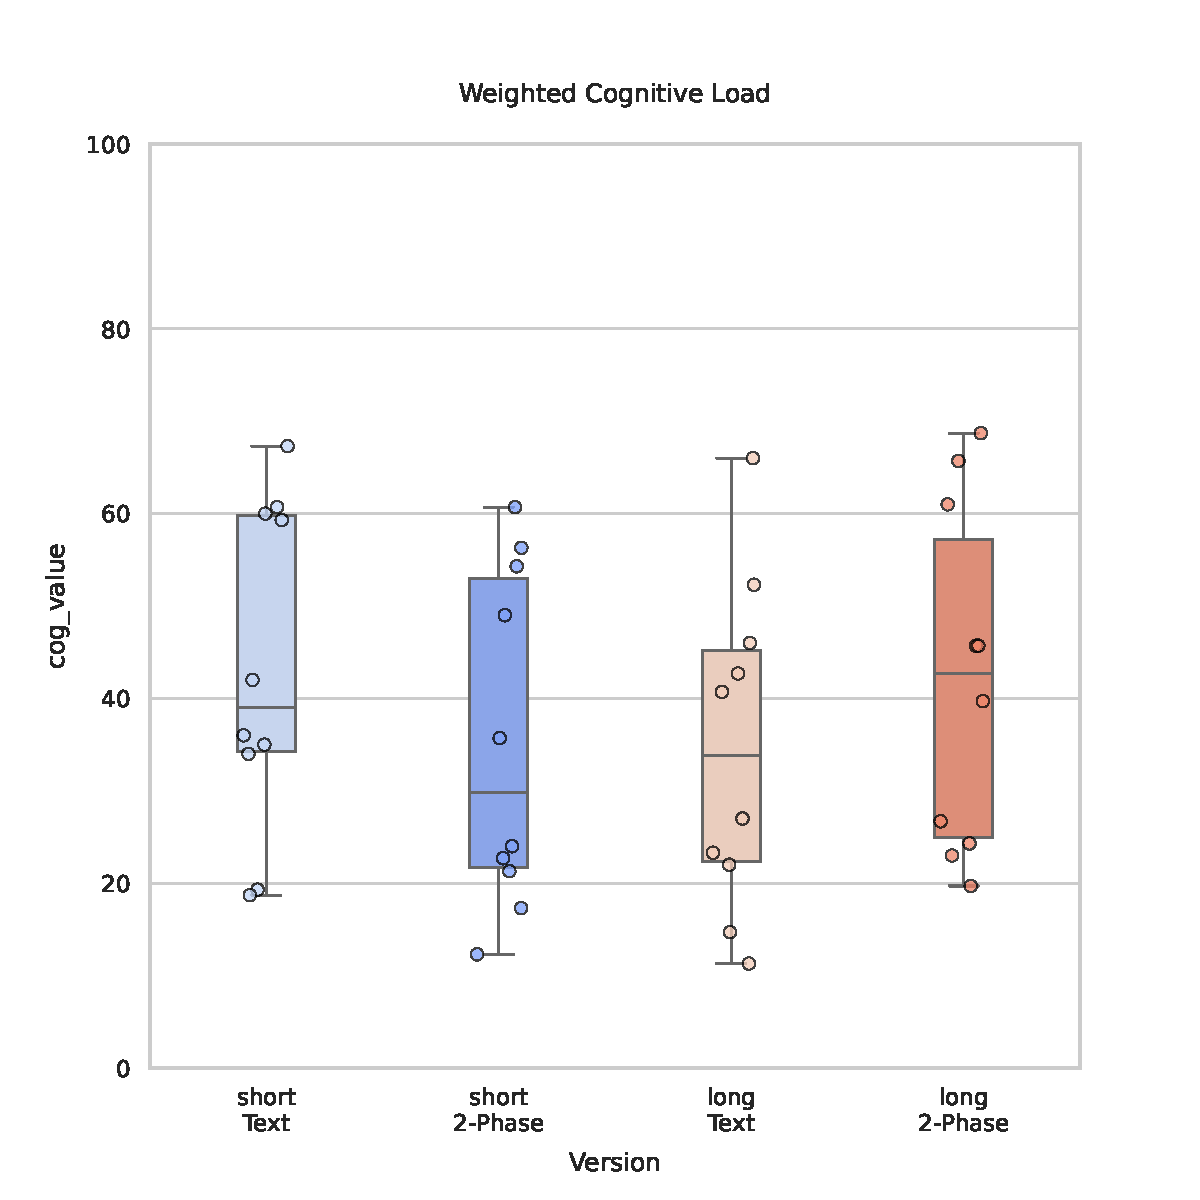
\includegraphics[width=\textwidth]{content/image/results/nasatlx_final_value.pdf}
        \caption{NASA-TLX Weight Score Distribution}
        \label{fig:nasatlx-final1}
    \end{subfigure}
    \hfill
    \begin{subfigure}[b]{0.47\textwidth}
        \centering
        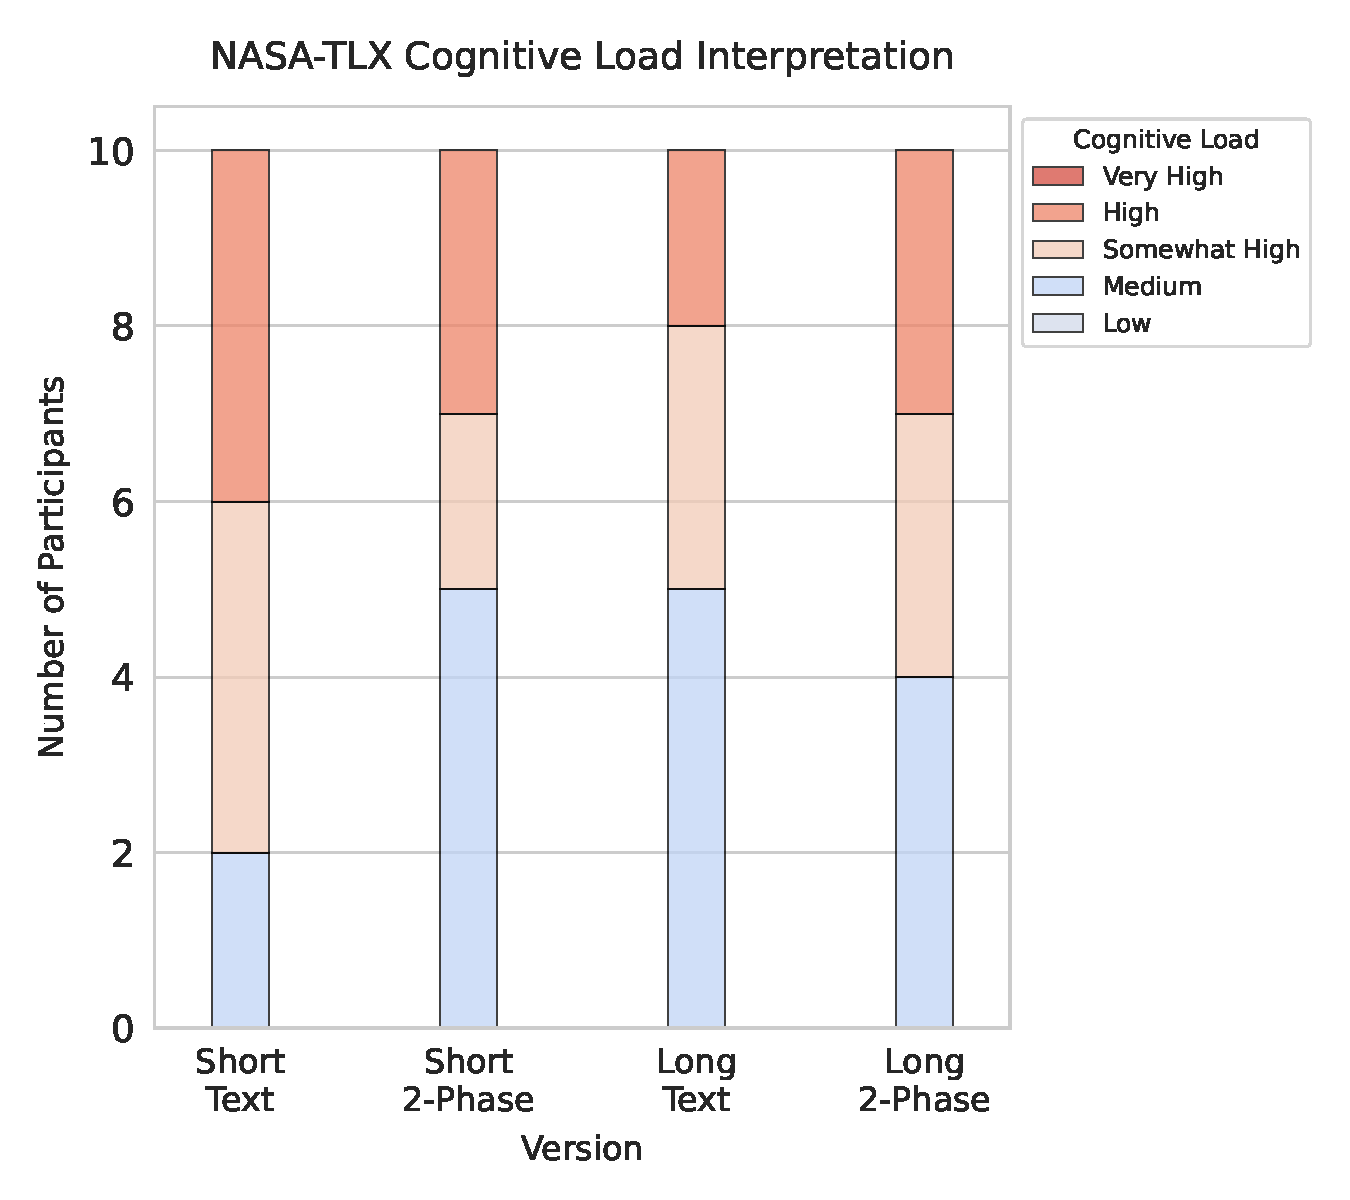
\includegraphics[width=\textwidth]{content/image/results/nasatlx_cog_value_interpreted.pdf}
        \caption{NASA-TLX Cognitive Interpretation}
        \label{fig:nasatlx-final2}
    \end{subfigure}
    \caption{NASA-TLX Results}
    \label{fig:nasatlx-final}
\end{figure}

We show the NASA-TLX weighted results in Figure~\ref{fig:nasatlx-final1}. A higher value refers to higher cognitive load. Qualitatively, the interactive interfaced decreased the cognitive load for the short survey, but seems to have increased the cognitive load for the long survey. A Mann-Whitney U-Test indicates that these differences are not statistically significant. We follow predefined mappings of NASA-TLX values to cognitive levels: low, medium, somewhat high, high, and very high, as listed by ~\textcite{hart1988development}. We show value interpretations in Figure~\ref{fig:nasatlx-final2}. The short text interface had the most participants ($N=8$) rating their cognitive experience as somewhat high or above. The other three experiment groups showed similar cognitive load with about half of the participants experiencing medium cognitive load and the others experiencing somewhat high or high loads. No participants in any conditions expressed experiencing very high cognitive loads.

These results partially answer our first two research questions. To our surprise, the longer survey did not introduce extraneous cognitive load despite the budget of the long QS increasing by 8 times and the options increasing fourfold. We deduct through a list of possible explainations. First, the interactive interface increases participants' cognitive load. However, we do not think this is the case. If it were, we would expect to see even more significant cognitive overload in the long interactive interface, resulting in lower cognitive load scores. Second, participants in the long text interface are cognitively overloaded, leading to satisficing behaviors due to the numerous decisions required to complete the task. We investigate if this is true in the following subsection. Third, we cannot rule out that the interface, contrary to our expectations, did not reduce cognitive load but rather shifts participants' cognitive load throughout the process of completing QS.

% TODO: MERGE INTO ABOVE PARAGRAPH :: Based on these results, given the small sample size for each group of participants, we were not surprised that most results do not provide statistical significance in changes in cognitive load values. However, there are some trends that we capture via descriptive statistics. First, comparing the overall cognitive load and the breakdown of the sub-components between text interface and interactive interface across the short survey, we see a general trend in a reduction of cognitive load. Next, we are surprised by the upward trend between the text and interactive interface for the longer list. This is against our original hypothesis that under even complex situations, we should see a clearer portrait of how interactive interactions can reduce cognitive load. While it is possible that interactive interfaces can increase study participants' cognitive load, our qualitative results do not hint at this possibility. In addition, comparing the long and short survey in the text-based interface, it is counter intuitive to see a downward trend across cognitive load. Logically, choosing among more options would demonstrate a higher cognitive load.

\begin{figure}[ht]
    \centering
    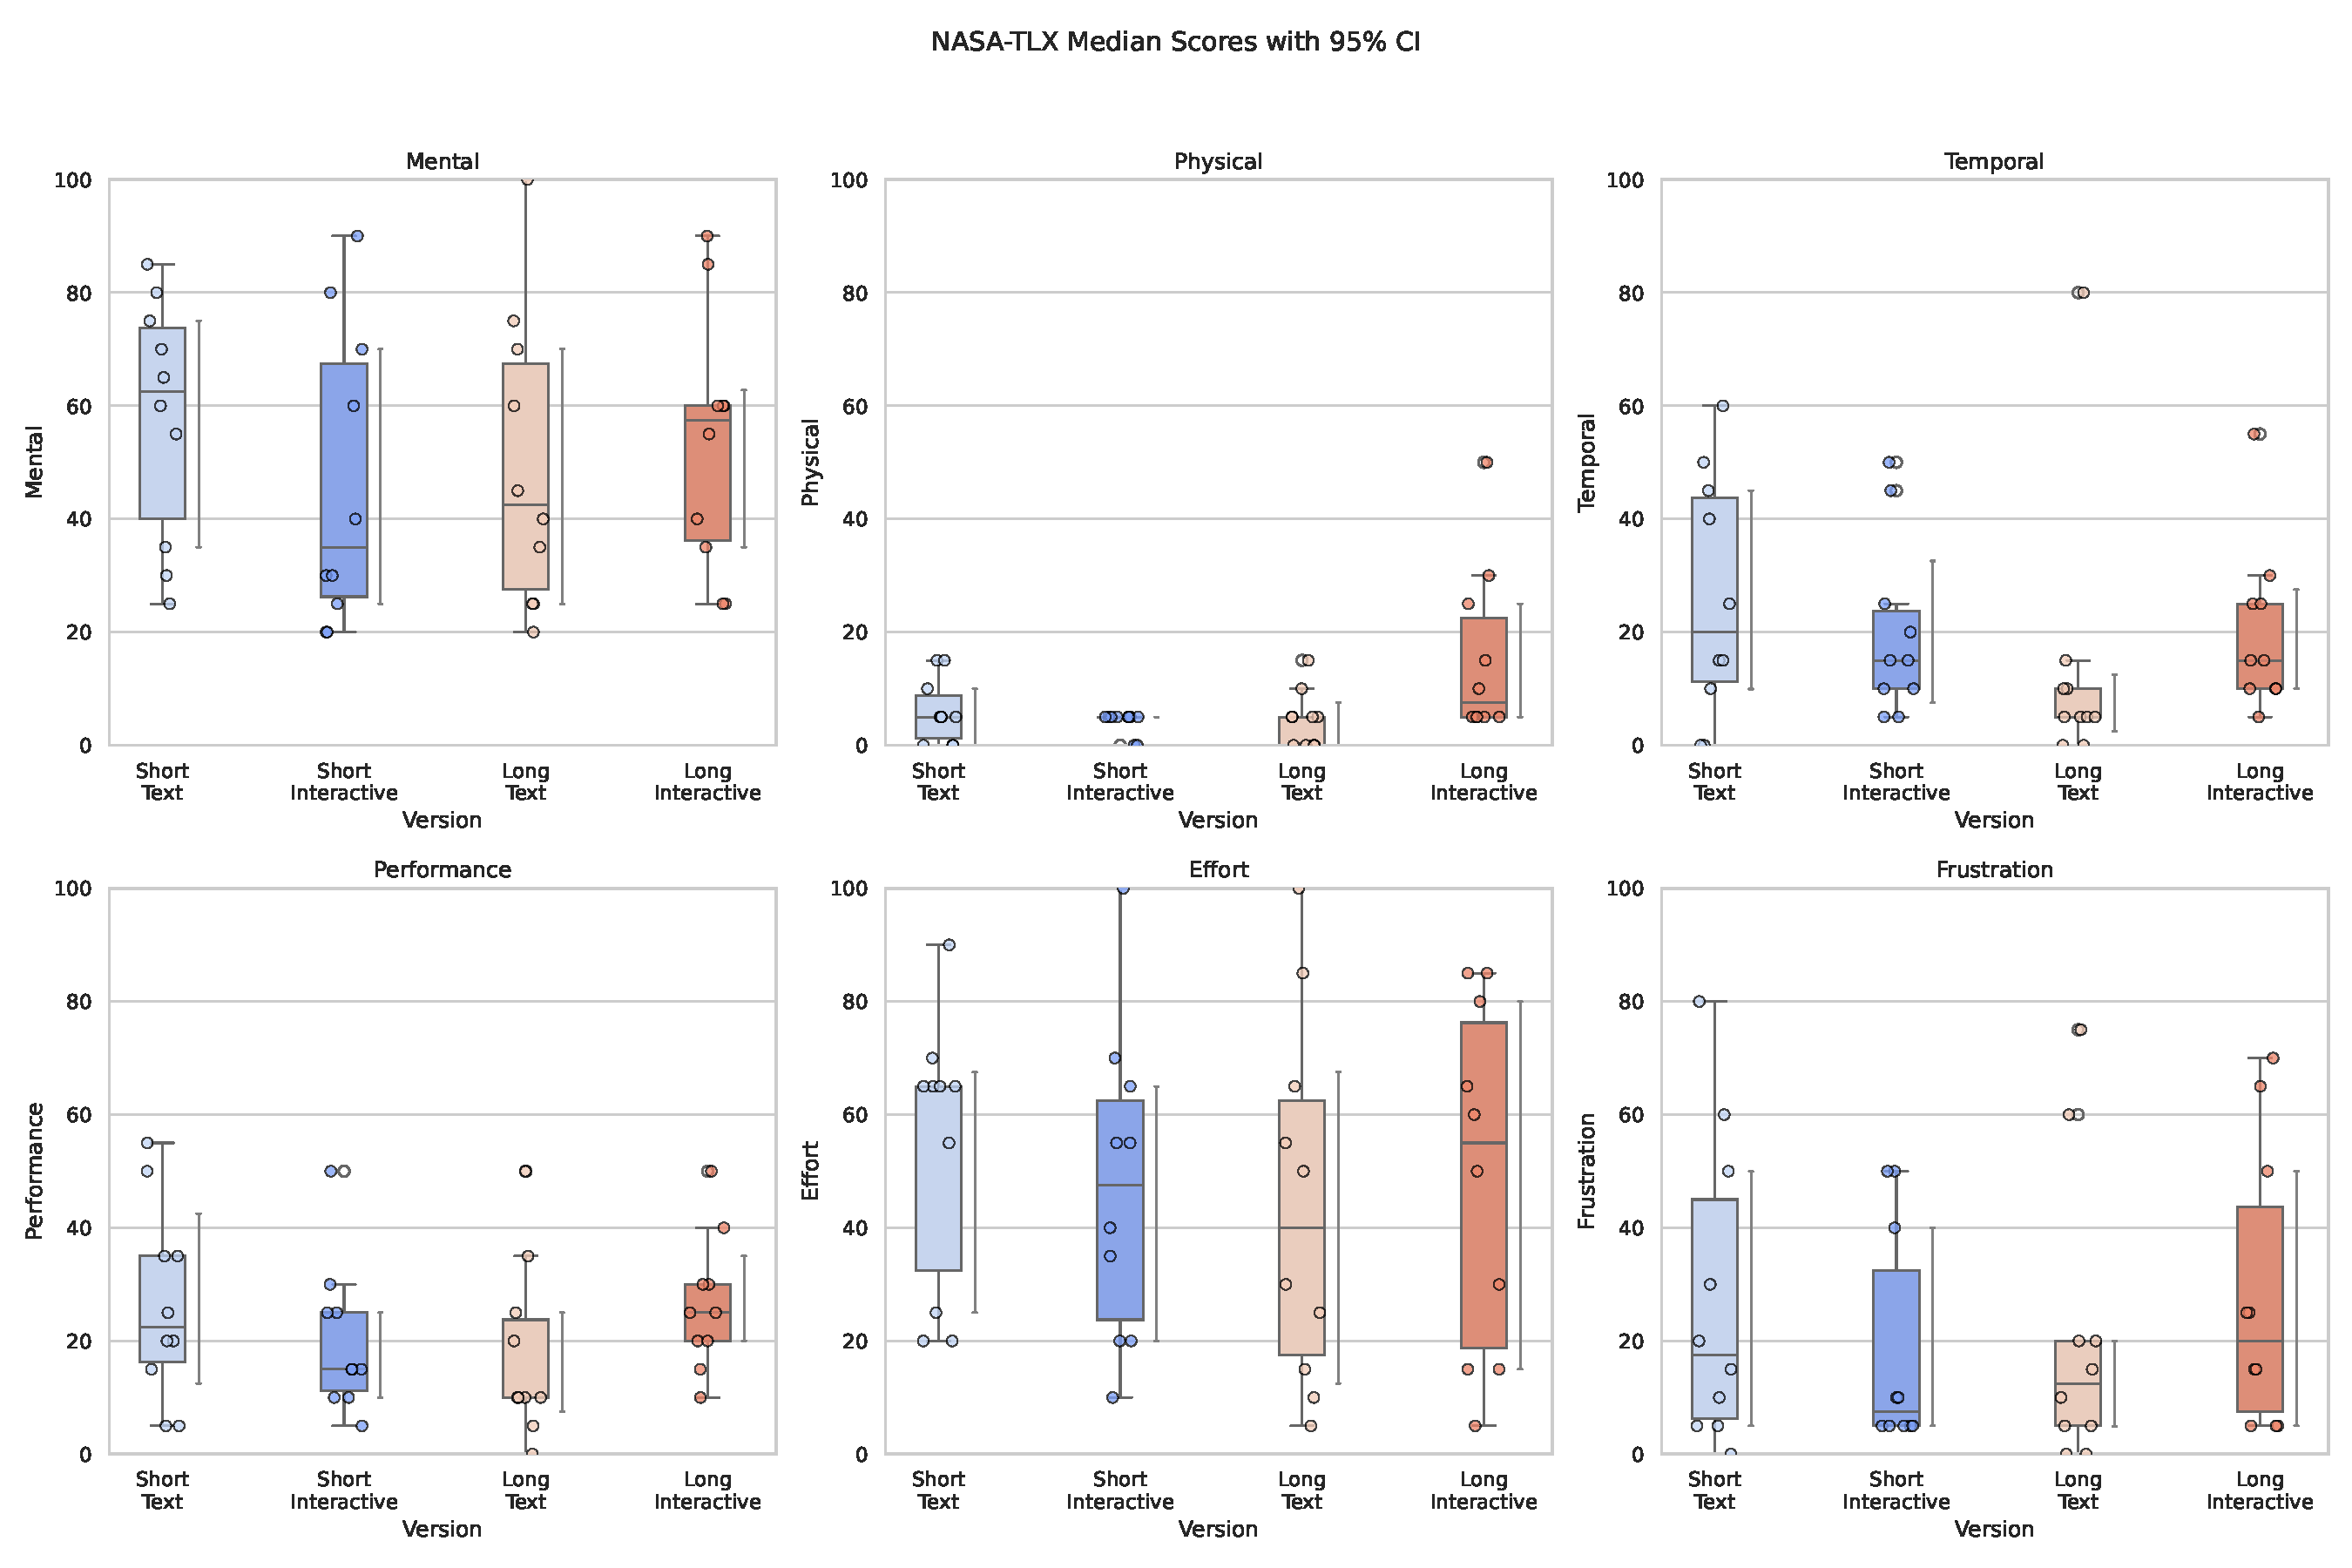
\includegraphics[width=\textwidth]{content/image/results/nasatlx_final_value_with_CI.pdf}
    \caption{NASA-TLX Results}
    \label{fig:nasatlx-with-ci}
\end{figure}


\subsection{Sources of Cognitive load}
NASA-TLX consists of six weighted dimensions: mental demand, physical demand, temporal demand, performance, effort, and frustration. To better understand the sources of cognitive demand and answer RQ2b, we highlight qualitative similarities and differences across four experiment conditions. This is followed by descriptive statistics and participant survey findings.

We present the raw NASA-TLX scale results in Figure~\ref{fig:nasatlx-with-ci}. Next to each box plot, a line is present to denote the 95\% confidence interval around the mean for each boxplot.

\subsubsection{Mental Demand}
Mental demand refers to the extent of mental and perceptual activity required. From the interview results, we identified two major sources contributing to mental demand:~\textit{Budget management} and~\textit{Preference construction}. Despite all experiment groups sharing these themes, we notice a distinct difference in the scope of~\textit{Preference construction}, especially when comparing long text and interactive interfaces.

\paragraph{Budget management} $17$ participants expressed demand from trying to budget within limited credit ($N=4$), track remaining credits ($N=10$), and maximize the use of credits ($N=8$). For example:

\begin{displayquote}
How many I got left that~\ldots\ that I haven't voted on yet, and seeing if I and looking at the remaining credits, I'm trying to mentally divide that up before I start allocating upvotes and downvotes.

\small{\noindent \hfill -- S006, long interactive interface}
\end{displayquote}

\begin{displayquote}
And then I just wanted to make sure that I used all the credit that I had available to me, and also knowing that in order to like show your support for certain societal issues you had to like that was giving a tangential take away from other societal issues that you could support as well.
    
\noindent \hfill -- S032, short text interface.
\end{displayquote}

In the first quote, the participant struggles with not running out of credit while allocating credits to options they haven't yet attributed. The second quote highlights the challenge of maximizing spend while ensuring sufficient differentiation. All these factors relate to effective budget management.

\paragraph{Preference construction} Almost all participants ($N=36$) experienced an increase in mental demand due to preference construction. This can be broken down into three sources: determining relative preference ($N=16$), where participants focus on internal evaluation and comparison among different options; option prioritization ($N=17$),  where participants make trade-offs to identify high-priority options and translate internal preferences into a subset of options; and precise resource allocation ($N=30$), where participants allocate specific values or adjustments to represent their preferences. For each of these sources, we show an example:

\begin{displayquote}
Figuring out my priorities, and how much I prioritize option 1 over option 2. What is the difference between those 2 on my priority list?

\hfill -- S002, short interactive interface, determining relative preference
\end{displayquote}

% I think the whole time I was trying to balance, I think II think I partly was discovering my what's the word I want to use bias isn't quite right. My priorities (S031, I)

\begin{displayquote}
I knew which ones that I wanted to dedicate the most to, and I knew which one I wanted to dedicate the least to. But it was that middle area that was kind of a grey area.
    
\noindent \hfill -- S008, short interactive interface, option prioritization
\end{displayquote}

% I knew which ones that I wanted to dedicate the most to, and I knew which one I wanted to dedicate the least to. But it was that middle area that was kind of a grey area.
% \noindent \hfill -- S024, short text interface, option prioritization

\begin{displayquote}
I'm not sure how to put into words~\ldots like having to pick how many upvotes would go to each one
    
\noindent \hfill -- S023, long text interface, precice resource allocation
\end{displayquote}

While these sources are common across all experiment groups, when we focus on participants in the long QS condition, the sources of preference construction showed different scopes between participants using text and interactive interfaces. More specifically, participants ($N=8$) in the long text interface tend to experience mental demand from preference construction by thinking about issues more narrowly and focusing on personal relevance. Conversely, participants ($N=9$) in the long interactive interface experience higher mental demand from considering the broader societal impact and evaluating options more holistically. Only four participants in the long text interface expressed a holistic view, and three participants in the long interactive interface expressed a narrow and personal view.

% \begin{displayquote}
% \bracketellipsis also seeing the long list and obviously having to pick between quite a few things that I do feel very strongly about and having to figure out which ones do, I feel more strongly about than others.
    
% \noindent \hfill -- S023, long text interface
% \end{displayquote}

\begin{displayquote}
Trying to figure out what upvotes I should give it you know~\ldots compared to~\ldots I even kind of went back compared to the other topics: <topic one> compared to <topic two>, and even with like <topic three>, I kind of went back and forth between those two. \bracketellipsis So it was very mental tasking for me.

\noindent \hfill -- S015, long text interface
\end{displayquote}

% \begin{displayquote}
% \bracketellipsis really having to think, especially with so many different societal issues. How do I personally prioritize them? And to what extent do I prioritize them?
    
% \noindent \hfill -- S009, long interactive interface
% \end{displayquote}

\begin{displayquote}
\bracketellipsis really going through the rest of the categories and deciding okay, which are the pressing issues of our time and which are the pressing issues for this particular society that that I live in. \bracketellipsis You know these causes need a lot more funding, and and others can probably still have some sort of an impact, even with less resources.

\noindent \hfill -- S019, long interactive interface
\end{displayquote}

In the first quote, participants expressed mental demand narrowly focused on three options, trying to recall specific characteristics to differentiate among the options. In the second quote, participants consider how options play a role in society and the bigger picture, aiming to maximize impact. While these differences seem subtle, they indicate a shift in cognitive load. It is possible that exposing participants to all options during the organizing phase forced them to think through all options.

Circling back to mental demand related to budget management across these two experiment conditions, we find that long text interface participants focused on more operational behaviors such as:

\begin{displayquote}
So I wanted to be fair.~\bracketellipsis I actually took my calculator out and said~\bracketellipsis  how much would it be if I equally distributed it and then how do I do that? Do I wanna do it all equally or not?

\noindent \hfill -- S020, long text interface
\end{displayquote}

compared to more procedures involving more strategic planning such as:

\begin{displayquote}
I wanted to make sure I wanted to give some credit to everything~\bracketellipsis I'm trying to make sure that I had without doing a lot of~\ldots I guess redos is trying to kind of get it right the first time on how I weight things.

\noindent \hfill -- S032, long interactive interface
\end{displayquote}

Strategic planning does not refer to gaming out others or 'winning' a game but rather to high-level thinking processes that consider strategies and plans to tackle a challenge, compared to operational tasks such as adjusting a specific vote value. While we did not notice significant differences in mental demand raw values (Figure~\ref{fig:nasatlx-with-ci}, top left figure) across the four experiment groups, the different actions regarding budget management and preference construction show a shift in mental demand across experiment conditions.

% IN_T4: Wanting more information on the options (N=6/40)
% 5. While the numbers seem small, non of this request came from v3. This could explain that participants are already overloaded from the existing the task.

% ============================================= %
\subsubsection{Physical Demand} Physical demand refers to the physical effort required to complete a task, such as physical exertion or movement. Since this study involves participants sitting in front of a computer screen completing a survey, most participants reported minimal physical demand. We nonetheless report the sources of this minimal demand, which include reading text on the screen ($N=4$), using the mouse ($N=16$), and moving their head to navigate the vertical screen ($N=5$). Participants emphasized that these demands were minimal, which is reflected in the low values reported in the NASA-TLX physical demand scores (Figure~\ref{fig:nasatlx-with-ci} middle top image.)
Notably, $11$ out of $20$ participants that used the interactive interface mentioned physical demand from using the mouse, reflecting their increased interaction with the interface. This is further supported by the raw NASA-TLX physical demand scores, which show statistical significance between short and long interactive interfaces ($p<0.01$) as well as between text and interactive interfaces in long surveys ($p<0.05$) after running a Mann-Whitney U test.

% ============================================= %
\subsubsection{Temporal Demand}
Temporal demand refers to the time pressure felt by the participant while performing a task. A lower temporal demand suggests participants experience a slow and leisurely pace.

The themes we uncovered from the interviews consist of three main sources that lead to participants' increase in temporal demand. These include:~\textit{Budget}, ~\textit{Decision Complexity}, and ~\textit{Operational Efficiency}. 

\paragraph{Budget}
Budget is a lightly discussed theme that emerged across experiment conditions. Four participants mentioned budget increasing their temporal demand. Although budget can only decrease through spending, it is interesting that some participants expressed that the reduction in credit value created a sense of time pressure. Participants translated the increasing marginal cost of votes into higher temporal demand. As one participant said,

\begin{displayquote}
When the money was decreasing, as I was casting more upvotes or downvotes so as the money decreases I felt kind of rushed.
            
\noindent \hfill -- S034, long interactive interface
\end{displayquote}

\paragraph{Decision Complexity} Decision Complexity refers to when participants felt that there are many decisions to make. These causes are expressed in two forms—affirmative and negative. Affirmative perception refers to participants explicitly expressing that there are many decisions to make, while negative perception refers to participants describing concerns regarding the time and effort already invested in the survey.

\begin{displayquote}
So it didn't take too much time but obviously there was a lot of things to consider. So there was some temporal demand.
    
\noindent \hfill -- S022, short interactive interface
\end{displayquote}

\begin{displayquote}
\bracketellipsis so at first it was like, `Okay, this is fine.' But then on the end, I was like, maybe I should just hurry up and make a decision. So it's like at first it would been here, but then I kinda moved up near the end when I was hanging a waffling between my upvotes.
\noindent \hfill -- S024, short text interface
\end{displayquote}

The former quote pointed out participants making many decisions , while the latter highlighted the increase in temporal demand due to an expected devoted time. What we found important was that each experiment group had participants expressing both perspectives on decision complexity as a source of temporal demand. However, half of the participants ($N=5$) in the short text interface and half of the participants ($N=5$) in long interactive interface expressed concerns due to decision complexity. The long interactive interface involved all five participants registering an affirmative perspective. This is not surprising because participants in the long interactive interface had the most actions needed for organizing and voting. On the other hand, it is interesting to observe that four of these five participants in the short text interface expressed a negative perspective. This indicates that participants in this group are highly sensitive to their sunk cost effect.
% v2 -- 2 and v3 -- 3

\paragraph{Operational Efficiency}
Unlike decision complexity, which refers to the abundance of decisions to be made, operational efficiency refers to specific and concrete operations or goals. For example, completing the survey, executing an operation, or accomplishing a specific task like updating vote values.

\begin{displayquote}
I wanna get through things in an efficient manner which doesn't necessarily mean I rush it. But it does mean that I do things expeditiously. Especially. I'd like to think I'm somewhat computer-savvy. And so to be able to move through this quickly and efficiently. I do take pride in, but it's all personal stuff. It's not nothing outwardly influencing me. 
        
\noindent \hfill -- S032, short text interface
\end{displayquote}

\begin{displayquote}
I want the credit done but I don't want to be overthinking.
            
\noindent \hfill -- S013, short text interface
\end{displayquote}

The former quote refers to the participant aims to operate swiftly on the interface, not specifically related to decision making. Similarly, the latter focuses on using the credit to complete a specific goal. When asked about temporal demand, 11 participants (five from interactive and six from text interface) out of 20 who responded to the short survey expressed operational efficiency resulting in temporal demand, compared to just five (three from text and two from interactive interface) out of 20 in the long interface group.

Taking~\textit{Decision Complexity} and~\textit{Operational Efficiency} altogether, we interpret that the participants in the short survey misperceived the task as simple, seeing just six options on the screen, and thus anticipated the task to be simple and easily completed. We observe similar patterns from the NASA-TLX temporal demand raw values (Figure~\ref{fig:nasatlx-with-ci}). The short text interface shows a relatively higher demand across the four groups, reflecting the demand from both decision complexity and operational efficiency. This is followed by the short interactive interface, affected by operational efficiency, and the long interactive interface, affected by decision complexity. The long text interface showed the least amount of temporal demand. Our statistical tests showed a significant difference between the long text interface and the long interactive interface ($p<0.05$) after a Mann-Whitney U test.

It is also worth noting that three participants from the 20 who responded to the long survey mentioned that the vertical screen's ability to see all options facilitated direct comparisons and transparency about the entirety of the task, which reduced the temporal demand.

\begin{displayquote}
(Seeing) all at once I can see how many there are, so it's kind of like I can kind of tell when I will be done.

\noindent \hfill -- S041, long text interface
\end{displayquote}

% ============================================= %
\subsubsection{Performance}
Performance refers to how the person perceived if they successfully completed the task. A lower value refers to a good performance and vice versa. We find less differences between experiment groups qualitatively and quantitatively. However, there are notable takeaways that we can derive from the data.

First, we identified two sources of performance demand:~\textit{Operational Actions} and~\textit{Social Responsibility} from the interviews. 

\paragraph{Operational Actions}
Similar to previous demands, operational actions refer to specific and executable procedures participants can perform in the survey. These sources are shared across experiment groups. Six participants reported feeling pressured to spend all their credits or ensure they stayed within budget. Five participants were concerned that their choices did not accurately reflect their true preferences. Additionally, six participants mentioned experiencing performance demand due to the limited time, energy, and resources available, which ties into other cognitive demands. Here we show two examples:

\begin{displayquote}
I don't think I did it perfectly, because I didn't have 0 remaining credits.
    
\noindent \hfill -- S024, short text interface, budget management
\end{displayquote}

\begin{displayquote}
I'm concerned that it's not as reflective of my views as I wanted to be like, or I was concerned about it.~\bracketellipsis I was concerned that maybe it didn't.

\noindent \hfill -- S041, long text interface, preference reflectiveness
\end{displayquote}

\paragraph{Social Responsibility}
Social Responsibility is a noteworthy source of perforamce demand, categorized into accounting~\textit{decision-maker responsibility} (N=8) and from considering~\textit{uncertainity of the outcome} (N=3). The former refers to individuals feeling guilty because they weren't able to avoid because of specific tradeoffs or that they want to be fair. For example, 

\begin{displayquote}
I don't want people to think that I just like don't care about <ethnicity> people at all. I also don't think like government funding should go towards like religious organizations. You know what I mean. So I don't want somebody to think that like, I just don't care about <ethnicity> people.
    
\noindent \hfill -- S041, long text interface, decision-maker responsibility
\end{displayquote}

In this quote, the participant placed themselves inside the shoes of a member of the government, rather than a citizen expressing their own attitudes. This shift in roles introduced the perforamce demand, however, it demonstrated that QS shared decision maker's dilemma to individual survey respondents. This characteristic extends to the latter which further to the participants trying to forsee an outcome:

\begin{displayquote}
If I was actually running a government funding~\bracketellipsis I don't know how this (the survey results) might actually affect people. Some of these things might be unpopular or bad, or have outcomes that I didn't forsee.
    
\noindent \hfill -- S027, short interactive interface, uncertainity of the outcome
\end{displayquote}

Similar to the previous source, social responsibility is also shared across experiment groups. Considering the raw NASA-TLX scores(Figure~\ref{fig:nasatlx-with-ci}), participants expressed similar levels of perforamce score. This aligns with the interview results where most participants felt positive about their final submission. This result is expected because the task is designed to reflect their preferences, not to measure performance. We further analyzed the types of satisfactory statements regarding performance.


We identified three types of satisfactory statements regarding self reported performance:
\begin{itemize}
    \item \textit{Did their best} refers to statements where a participant stated they exhausted their maximum effort to complete the task.
    \item \textit{Feel good} efers to statements where a participant who expressed positive emotions or satisfaction about their performance or the outcome.
    \item \textit{Good enough} refers to statements where a participant acknowledged that their performance or the outcome was acceptable or satisfactory, but not necessarily perfect or the best possible.
\end{itemize}

We found approximately the same number of participants in each of the four experiment groups expressed \textit{Good enough}. Meanwhile, participants using the interactive interface across short and long groups had almost double the number of participants ($N=11$) who expressed \textit{Feel good} compared to the text interface ($N=6$). On the other hand, the text interface had slightly more participants ($N=5$) who expressed \textit{Did their best} compared to the interactive interface ($N=3$).

This result highlights a few important takeaways. First, participants from all experiment groups expressed satisficing behaviors (\textit{Good enough}) with no particular group reporting a higher frequency of this behavior. Second, participants using the text interface are experiencing challenges that make them feel they have to do their best to complete the task. Last, participants using the interactive interface are generally positive about their experience and the outcome.

% TODO: Need to check the reflective thinking part a bit. I **think** there are differences but it is unclear, need to go back to raw code.


% ============================================= %

\subsubsection{Effort}
Effort refers to the amount of work required to achieve a level of performance. It includes the intensity of both mental and physical resources expended during the task.

Similar to our analysis for mental demand, we code the source of effort into to major categories:~\textit{Operational Tasks} and~\textit{Strategic Planning}.

\paragraph{Operational Tasks} Similiar to performance, we focus on operational tasks that contributed to effort with a narrow focus including: navigating the interface, managing the budget at an operational scale (i.e., making sure not to run out of budget, making specific updates between two options), or translating an opinion to a quantifiable adjustment on the survey. These narrower low level operations involves taking effort to making updates or actions related to the interface itself. We show two examples associated with different aspects of operational tasks that influence precieved effort:

\begin{displayquote}
And then I wanted to bump up (an option) maybe to 4 or <option> to 5 and realize I couldn't. My point (number of votes) had to like back down a little bit~\ldots So that would be effort came in of how do I want to really rearrange this to make it (the budget spending) maximize?

\noindent \hfill -- S029, short text interface
\end{displayquote}

\begin{displayquote}
So it was like it was very~\ldots I have to put a lot of effort in terms of you know~\ldots think about each dimension that if I give one credit to <option name> whether it will affect my credits on <another option name>.

\noindent \hfill -- S005, long text interface
\end{displayquote}

Notably, $14$ of the $20$ participants using the text interface expressed overwhelminly mentioned sources related to such sources, compared to less than half of the participants ($N=7$) from the interactive interface, with the lowest mention by the long interactive interface group ($N=2$). We review the other category before making interpretations.

\paragraph{Strategic Planning} Opposite to operational tasks, strategic planning follow definitions established for mental demand which involces higher level strategies to complete the survey. We further derive two distinct types of planning:~\textit{personal} and~\textit{global}.~\textit{Personal strategic planning} refers to taking effort to translate preferences onto the survey without considering governing values or broader beliefs. For example, this participant expressed effort from retrieving past experiences to inform their decisions:

\begin{displayquote}
~\bracketellipsis having that prior experience and being able to quickly link it to a tangible thing that I've experienced in my personal life.

\noindent \hfill -- S032, short text interface
\end{displayquote}

\begin{displayquote}
And really the bulk of the effort was how to rank order these (options) and allocate the resources behind the upvotes so that I can accurately depict what I want~\ldots say, a committee to focus on and allocate actual fungible resources, too. 

\noindent \hfill -- S019, long interactive interface
\end{displayquote}

While the difference in the number of citations to personal strategic planning are less pronounced across groups, the interactive interface (N=13) still scores slightly higher counts compared to the text interface (N=9).~\textit{Global strategic planning}, on the other hand, involves participants formulating strategies to align with broader, communal values. This includes ensuring fairness, considering the impact of different options on the entire community, and evaluating the complex relationships between various options. For example:

\begin{displayquote}
I think, imagining the trying to imagine every outcome trying to to imagine what what else would be encompassed, encompassed by each category.

\noindent \hfill -- S027, short interactive interface
\end{displayquote}

\begin{displayquote}
Hey, even though I don't really like this idea. But what if they're important? They sort of kind of deserve some attention~\ldots that's why I think I have the effort here.

\noindent \hfill -- S037, long interactive interface
\end{displayquote}
    
Both examples shows considerations beyond personal experiences, considering outcomes or social values. We notice that nearly twice as many participants (N=7) in the interactive interface expressed effort from global strategic efforts compared to the text interface (N=4). Altogether, we observe more participants using the interactive interface (N=17) reported sources of strategic effort compared to those using text-based interfaces (N=11). 

Qualitative analysis in this subsubsection added clear evidence that the source of cognitive demand for effort differs between text and interactive interfaces, similiar to mental demand. Participants using the interactive interface focus less on operational tasks and more on strategic planning, specifcially global strategic planning, where they think about options holistically and beyond the option itself. This is in contrast to participants using the text interface, who focus more on operational tasks and a narrower strategic planning scope. The raw NASA-TLX effort scores (Figure~\ref{fig:nasatlx-with-ci}) can then be explained that even though reported values are similar across the four experiment groups, the sources of effort differ between text and interactive interfaces.

% ============================================= %

\subsubsection{Frustration}
Fustration is the last dimension of NASA-TLX. It refers to the extent to which the participant is annoyed, irritated, or discouraged during the task.

Following the previous analysis, we categorize the sources of frustration into three major themes:~\textit{Operational Actions} and~\textit{Strategic Planning}

\paragraph{Operational Actions} Similar to the previous definitions, $15$ participants highlighted this source for frustration. Six participants expressed frustration regarding credit management (i.e., overspending budget); four participants mentioned had trouble deciding the final value for the options; three participants are frustrated because they need to make multiple decisions; five participants were frustrated with the quadratic mechanism; four participants are frustrated trying to understand the content of the option or how the option connects to them. For example, 

\begin{displayquote}
I was slightly frustrated when doing the task, probably because there was a budget that we kind of had to stick with it.

\noindent \hfill -- S001, long text interface, quadratic mechanism
\end{displayquote}

\begin{displayquote}
i think just frustration~\bracketellipsis because when i was making like the decisions on how many upvotes I could put in each section, I was running out of credits.

\noindent \hfill -- S013, short interactive interface, budget management
\end{displayquote}

These demonstrated participants frustration because they are hindered by not being able to complete specific operational actions or constraints presented by QS. What is noteable is that all experiment groups had almost half of the participants express operational frustration compared to only two participants from the long text interface group. It is not clear why they did not encounter similiar frustration.

\paragraph{Strategic Planning} For frustration, we further derived strategic planning into two types: ~\textit{lower-level} and~\textit{higher-level}. For the former, Four participants expressed conflict between their personal preferences and what they believe would be other people's preferences. Eight participants experienced conflict between making tradeoffs among a few options. For example:

\begin{displayquote}
Because I know that's important to other people. But it just doesn't to me.
    
\noindent \hfill -- S010, short interactive interface
\end{displayquote}

\begin{displayquote}
I would have loved to have given more to other groups~\ldots and I felt stressed like~\bracketellipsis well~\ldots it's a group that you know is still~\ldots you know~\ldots important~\bracketellipsis
\noindent \hfill -- S020, long text interface
\end{displayquote}

These quotes showed participants trying to ahere to lower-level strategies such as considering personal prefernces or making trade-offs within a smaller scope. Compare to~\textit{higher-level strategic planning}, where six participants expressed conflicts that touch on the broader society and their core values of looking at the broader scope. Eight participants felt frustrated because they were forced to make trade-offs among \textit{all} options instead of a few. For example,

\begin{displayquote}
I had to consider how I feel towards that~\ldots how religious media broadcasting is being used in like today's society~\ldots today's political environment. So yeah~\ldots you really have to consider what is important to you. 
\noindent \hfill -- S020, long text interface, value conflicts
\end{displayquote}

\begin{displayquote}
I think the frustration is~\ldots I wish that we could help all of these causes, but you know it's just like anything else. You can't do everything and when it's not~\ldots  I feel like it's hard to quantify how much some of these things should be supported versus others. So when you're talking about upvotes and things that's challenging to me, it's frustrating.
\noindent \hfill -- S026, long interactive interface, considering all options
\end{displayquote}

Fustration that stemmed from strategy planning are spread across all experimental conditions. Reflecting on the raw NASA-TLX scores (Figure~\ref{fig:nasatlx-with-ci}), We only see a slight difference in less frustration from the long text interface participants compared with the rest of the participants, likey due to the less frustration from operational tasks. Thus, we interpret that frustration comes more from individual's ability to discern and make decisions and not necessarily tied to specific methods in the construction of preference.

\subsubsection{Summary}
% TODO: make a table
To recap, the analysis identified the different sources of cognitive load experienced by participants. More specifically, it highlighted differences across experimental conditions. Interactive interfaces, especially long ones, drive participants to adopt a holistic view and encourage higher-level deliberation, indicated by increased mental demand and effort. Conversely, participants perceived more operational demand when completing specific tasks using the text interface. Mental demand, effort, and temporal demand highlighted the urgency participants felt to complete tasks swiftly. This distinction doesn't mean one group of participants excludes the other group's demands, but it highlights that the main source of demand shifts with different interfaces.

% ============================================= %
\afterpage{
\begin{landscape}
    \begin{figure}[ht]
        \centering
        \begin{subfigure}[b]{0.26\pdfpageheight}
            \centering
            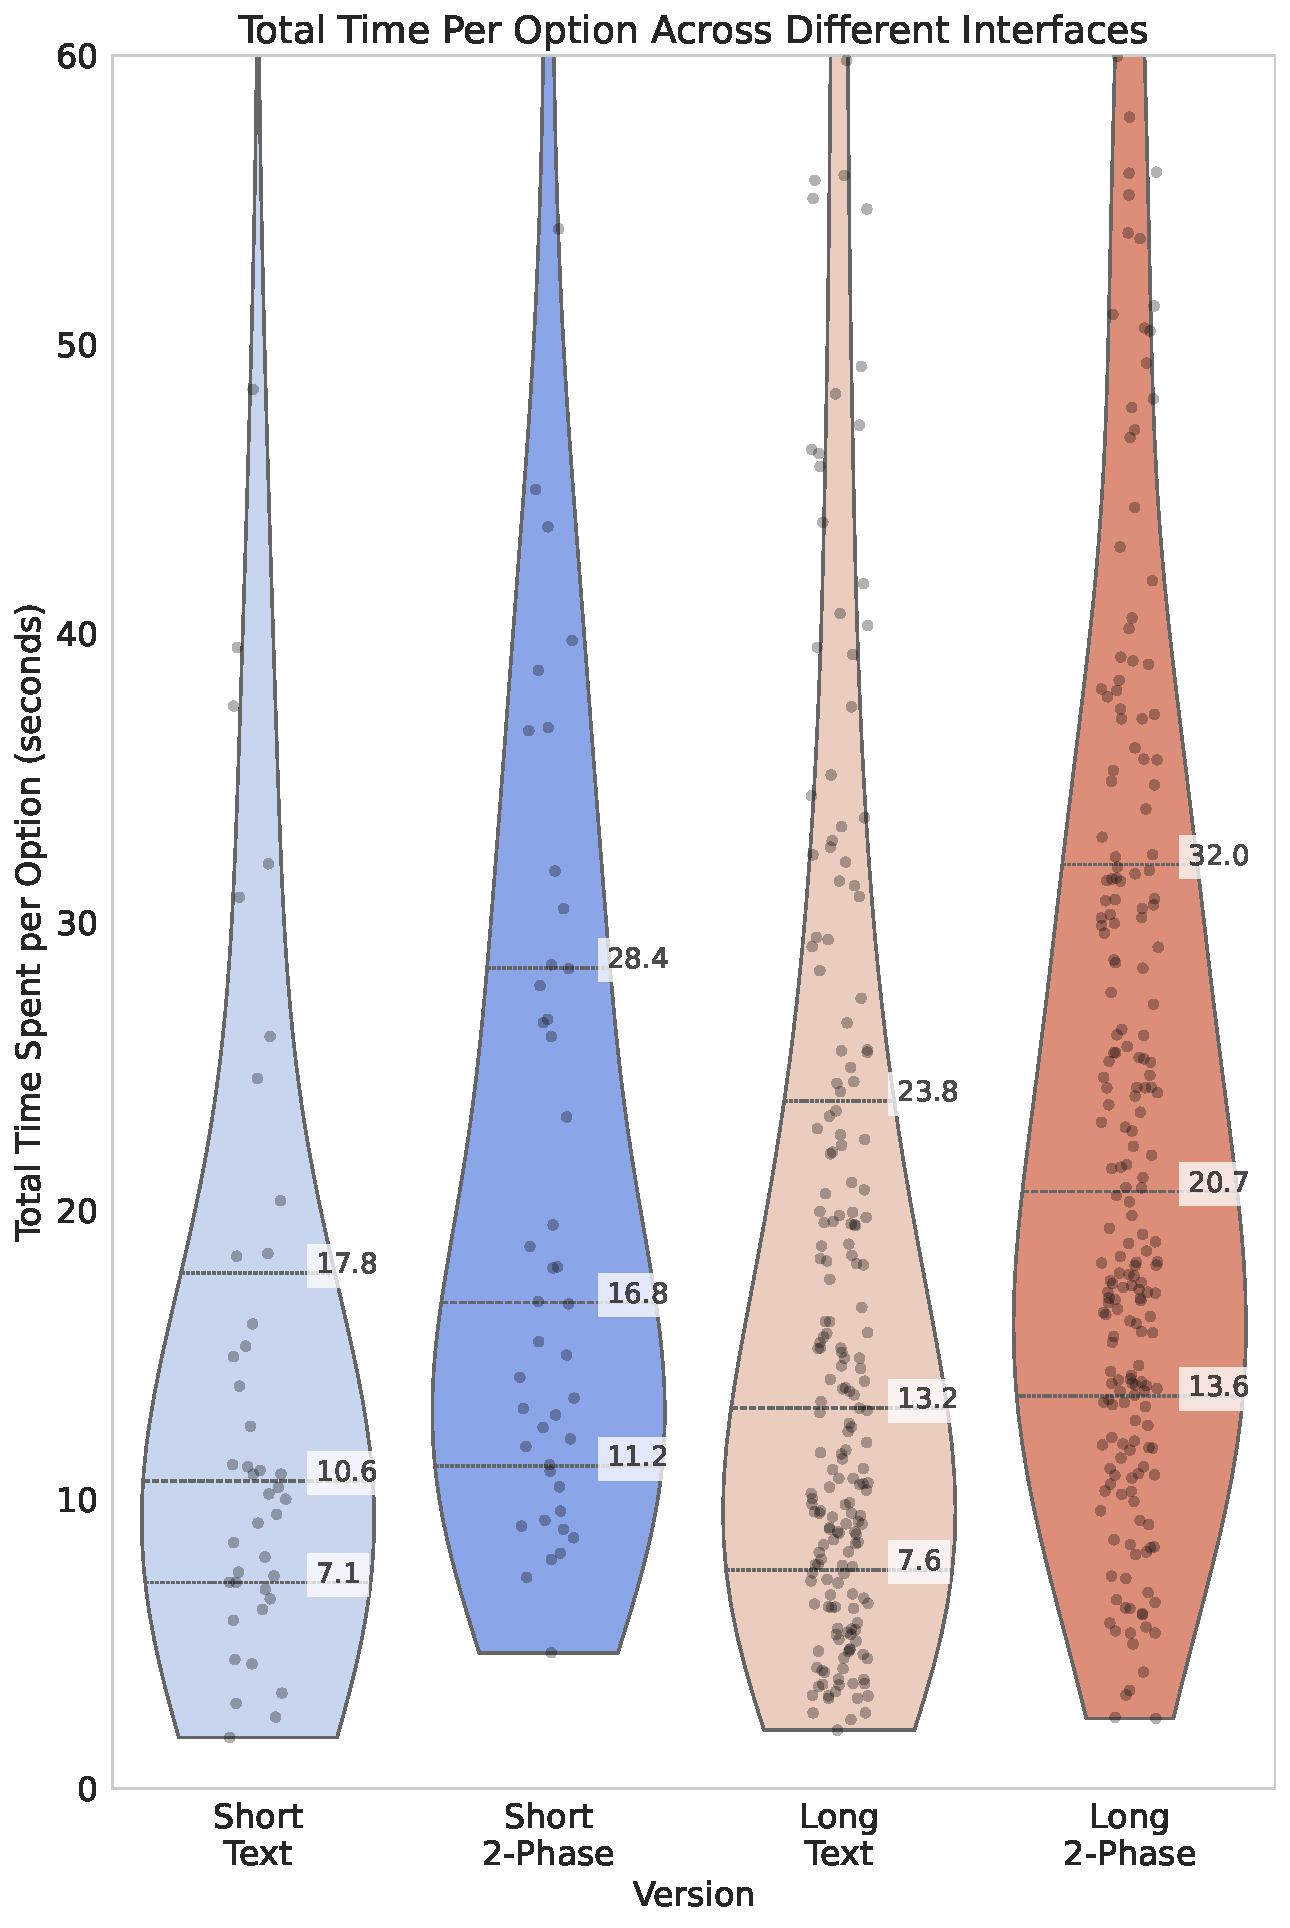
\includegraphics[width=\textwidth]{content/image/results/total_time_per_option.pdf}
            \caption{Total Time per option}
            \label{fig:total_time}
        \end{subfigure}
        \hfill
        \begin{subfigure}[b]{0.26\pdfpageheight}
            \centering
            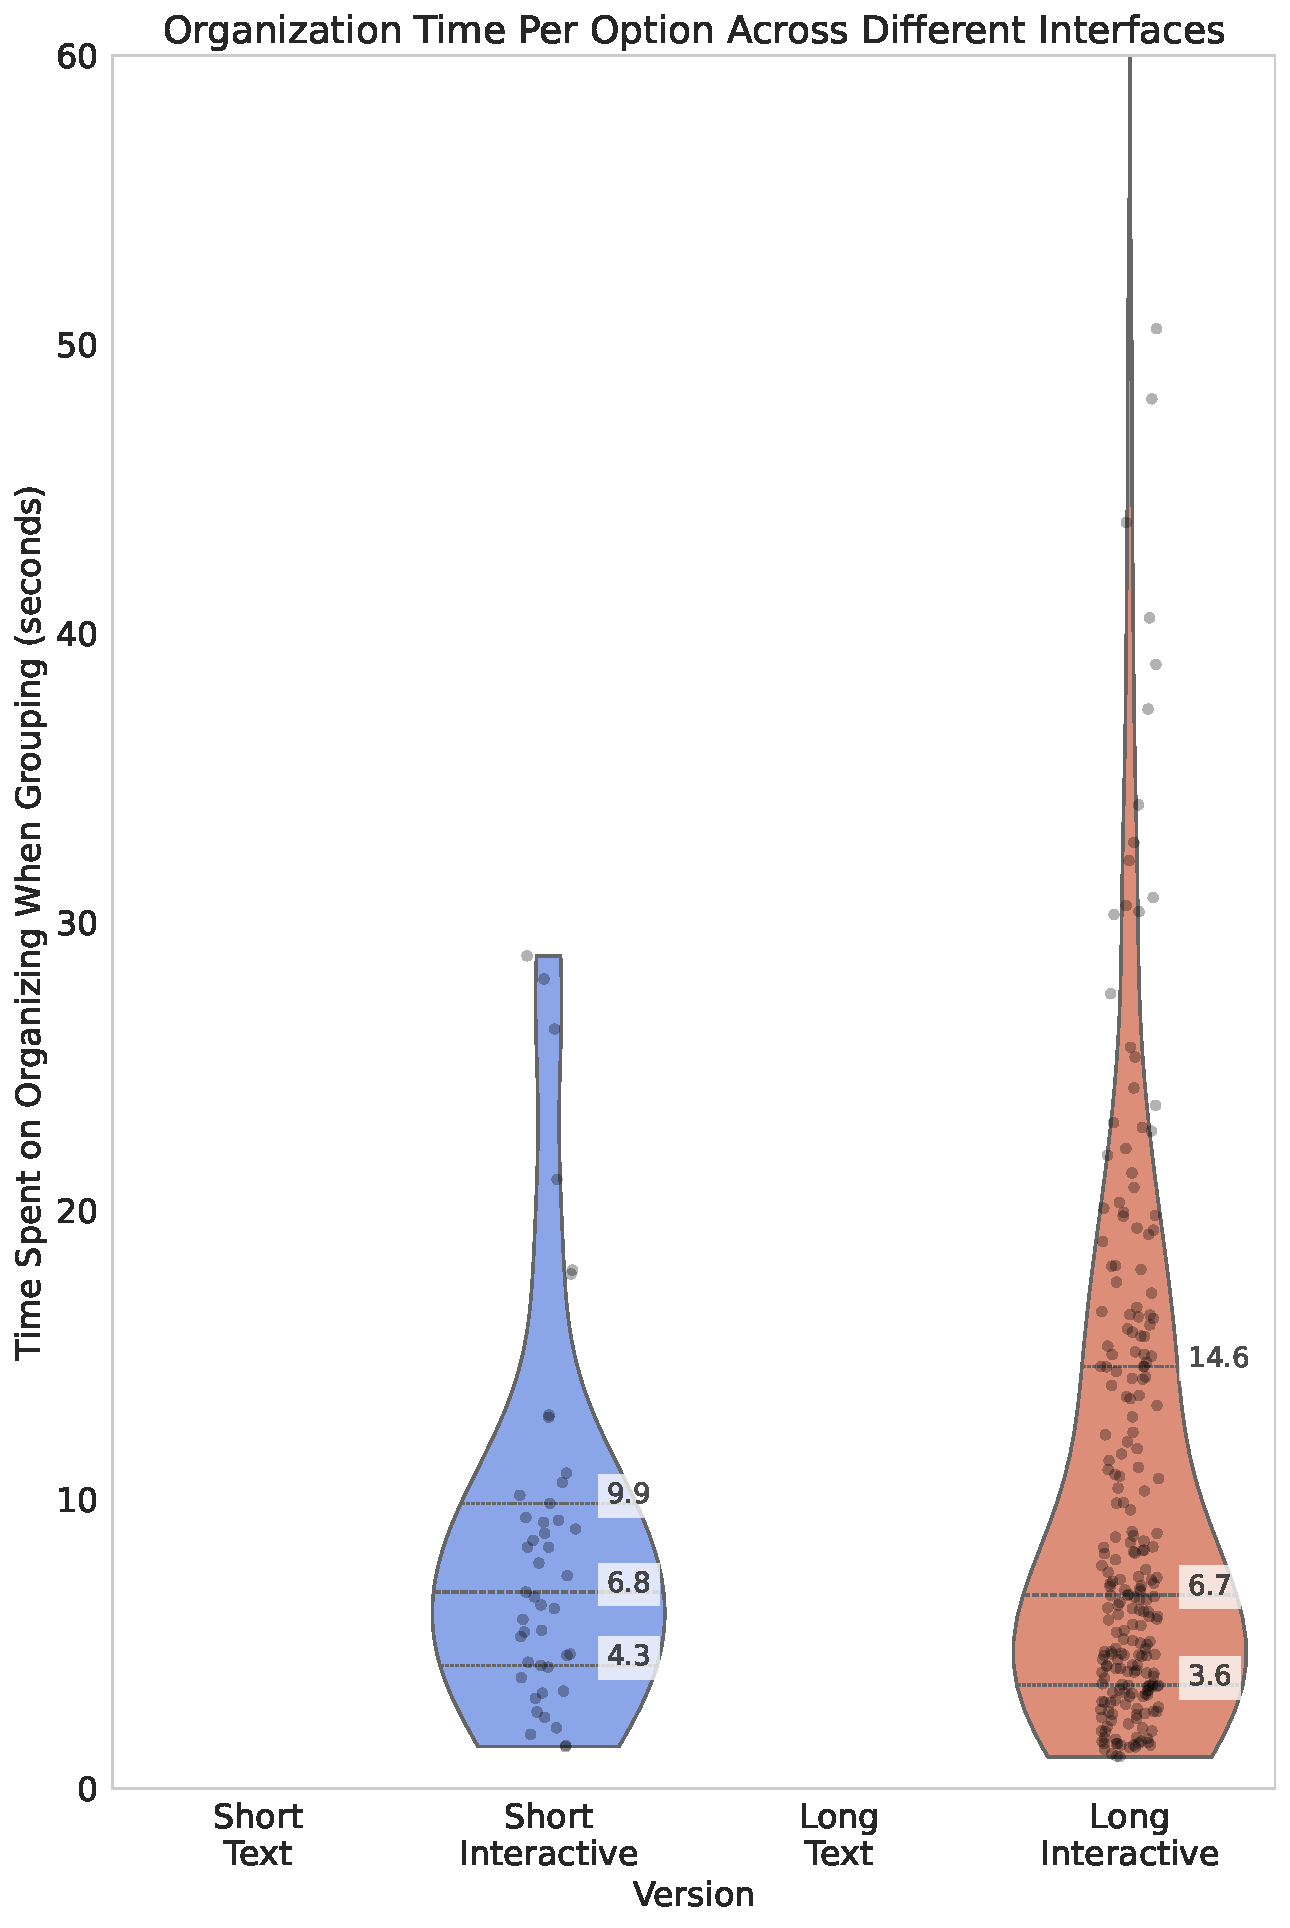
\includegraphics[width=\textwidth]{content/image/results/org_time_per_option.pdf}
            \caption{Organization Time per option}
            \label{fig:org_time}
        \end{subfigure}
        \hfill
        \begin{subfigure}[b]{0.26\pdfpageheight}
            \centering
            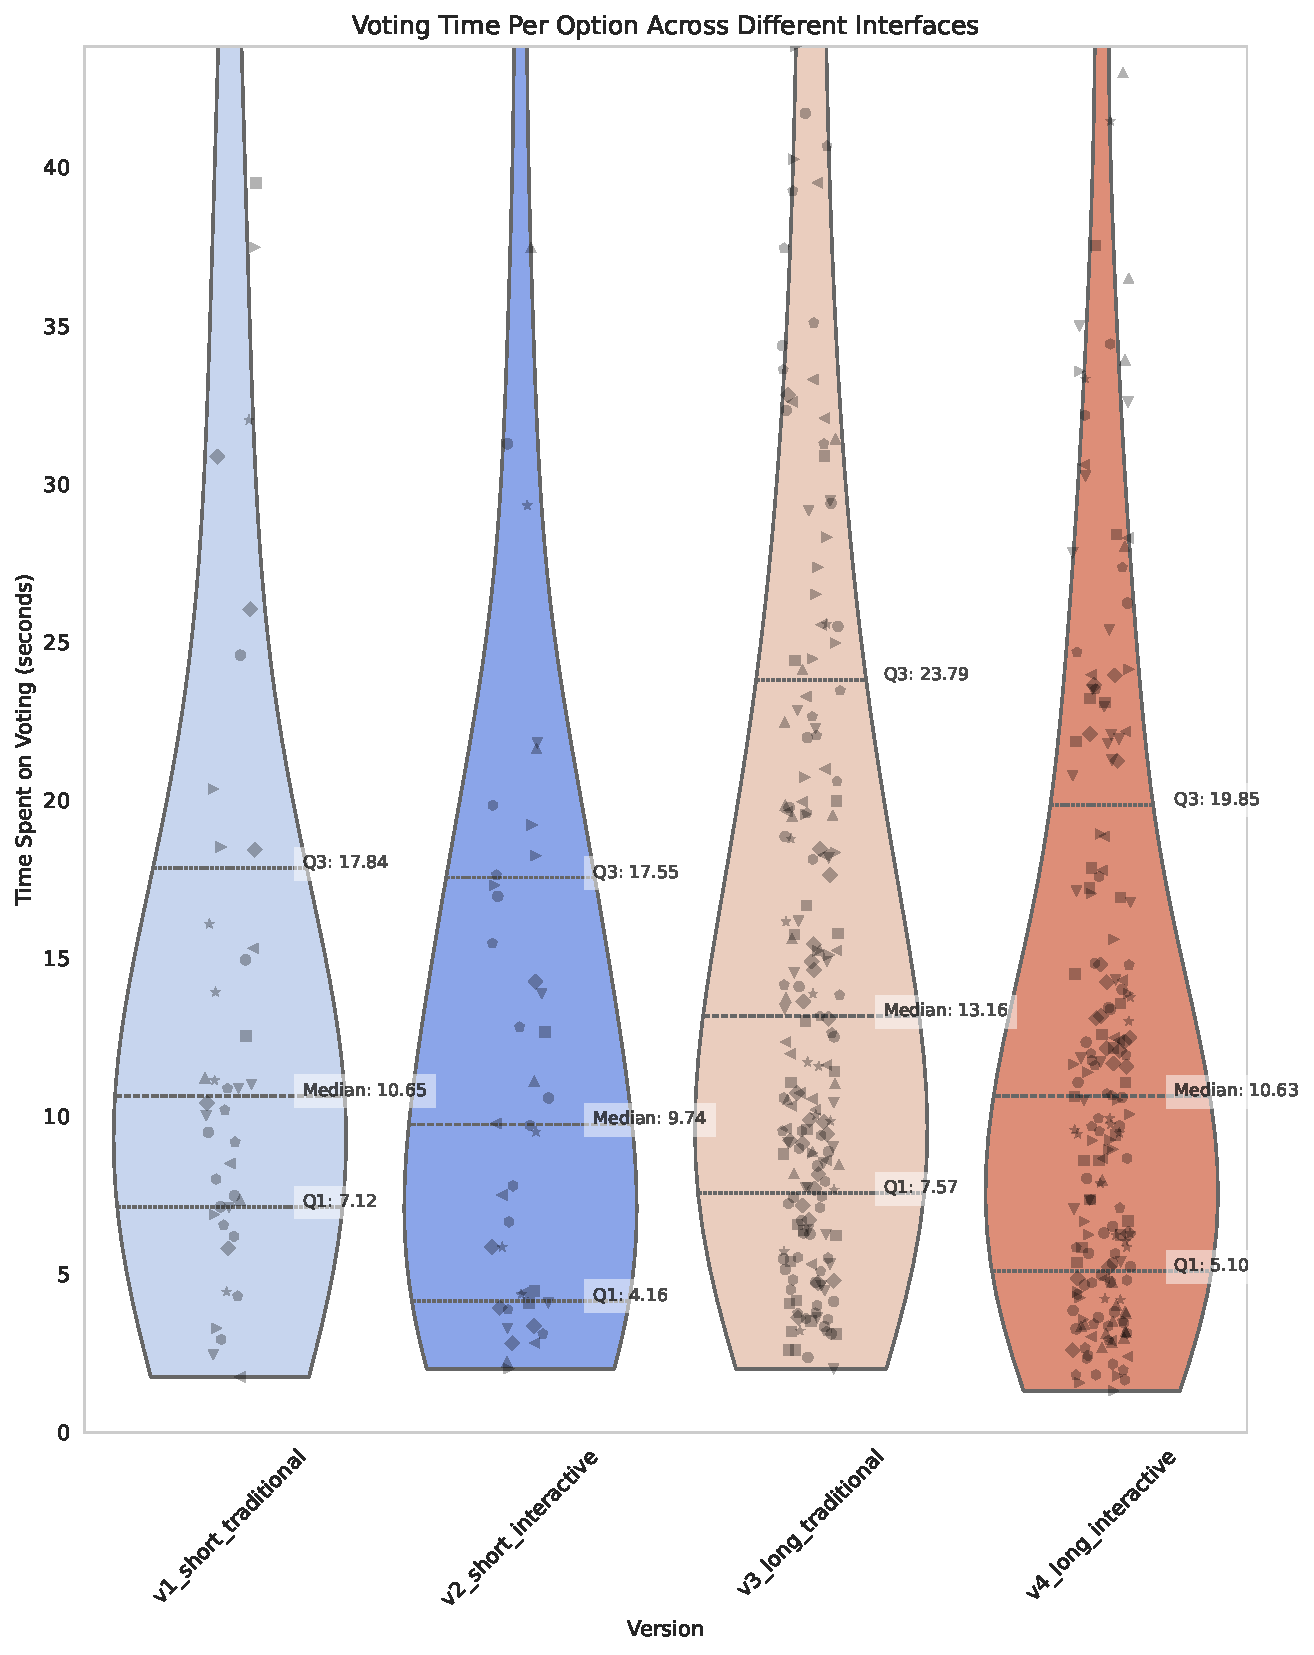
\includegraphics[width=\textwidth]{content/image/results/voting_time_per_option.pdf}
            \caption{Voting Time per option}
            \label{fig:vote_time}
        \end{subfigure}
        \caption{Breakdown of time per option}
        \label{fig:Time Spent Per Option Per Person}
    \end{figure}
\end{landscape}
}

\subsection{Interaction Behavior Analysis}
\label{sec:act}
To answer RQ3 and collect evidence of shifts in participants' cognitive sources, we analyze their behaviors during the survey. We aim to understand the time participants spend on options and when they make changes. When a participant clicks their mouse on the interface to complete an action, such as drag-and-drop, updating votes, or placing options into a specific group, a timestamp and the payload of the update are stored in the log. In this subsection, we analyze these log data. We acknowledge that the time difference between two actions indicates the time the participant took to decide and act. Although participants might be thinking about other things, this is our best proxy to study their behaviors.



\subsection{Time Spent per Options}
First, we define time spent per option. A participant can enact several actions related to the same option, for example, a participant might spend $t_1$ time to place the option into a `lean positive' category; spend $t_2$ and $t_3$ time to drag and drop the options to reposition it on the interactive interface; spend $t_4$ and $t_5$ time to update the upvotes on that option. In this case, we would define voting time as $t_4 + t_5$ for that option, and organization time as $t_1 + t_2 + t_3$.

To reduce noise, we intentionally drop all the time participants spent on the first option in the organization phase or voting phase. The goal is to reduce the inclusion of time they spent on reading the prompt, forming their preference, or understanding the interface. We present the results in Figure~\ref{fig:Time Spent Per Option Per Person} where each of the dots represents the time accumulated for an option that a participant interacted with. The violin plot shows the distribution of the dots and the three horizontal lines represent the median, 25th percentile, and 75th percentile of the time spent for that interface.

In Figure~\ref{fig:total_time}, we observe that participants spent more time on the interactive interface than the text interface in both short and long surveys. A non-parametric statistical test supports such observation with $p<0.01$ for short and $p<0.0001$ for long surveys. This is not surprising because participants need to review the options and organize them in the interactive interface which takes more time. We break down the total time spent into organization time and voting time in Figure~\ref{fig:org_time} and Figure~\ref{fig:vote_time}.

Once we separate the organization time (Figure~\ref{fig:org_time}) and identify the voting time (Figure~\ref{fig:vote_time}), while there are no statistically significant differences between the text interface and the interactive interface in the short survey, we see a statistically significant reduction ($p<0.01$) in voting time between the text interface and the interactive interface. In other words, our original hypothesis holds in which the two-step design process did facilitate participants in making their decisions.

\begin{figure}[ht]
    \centering
    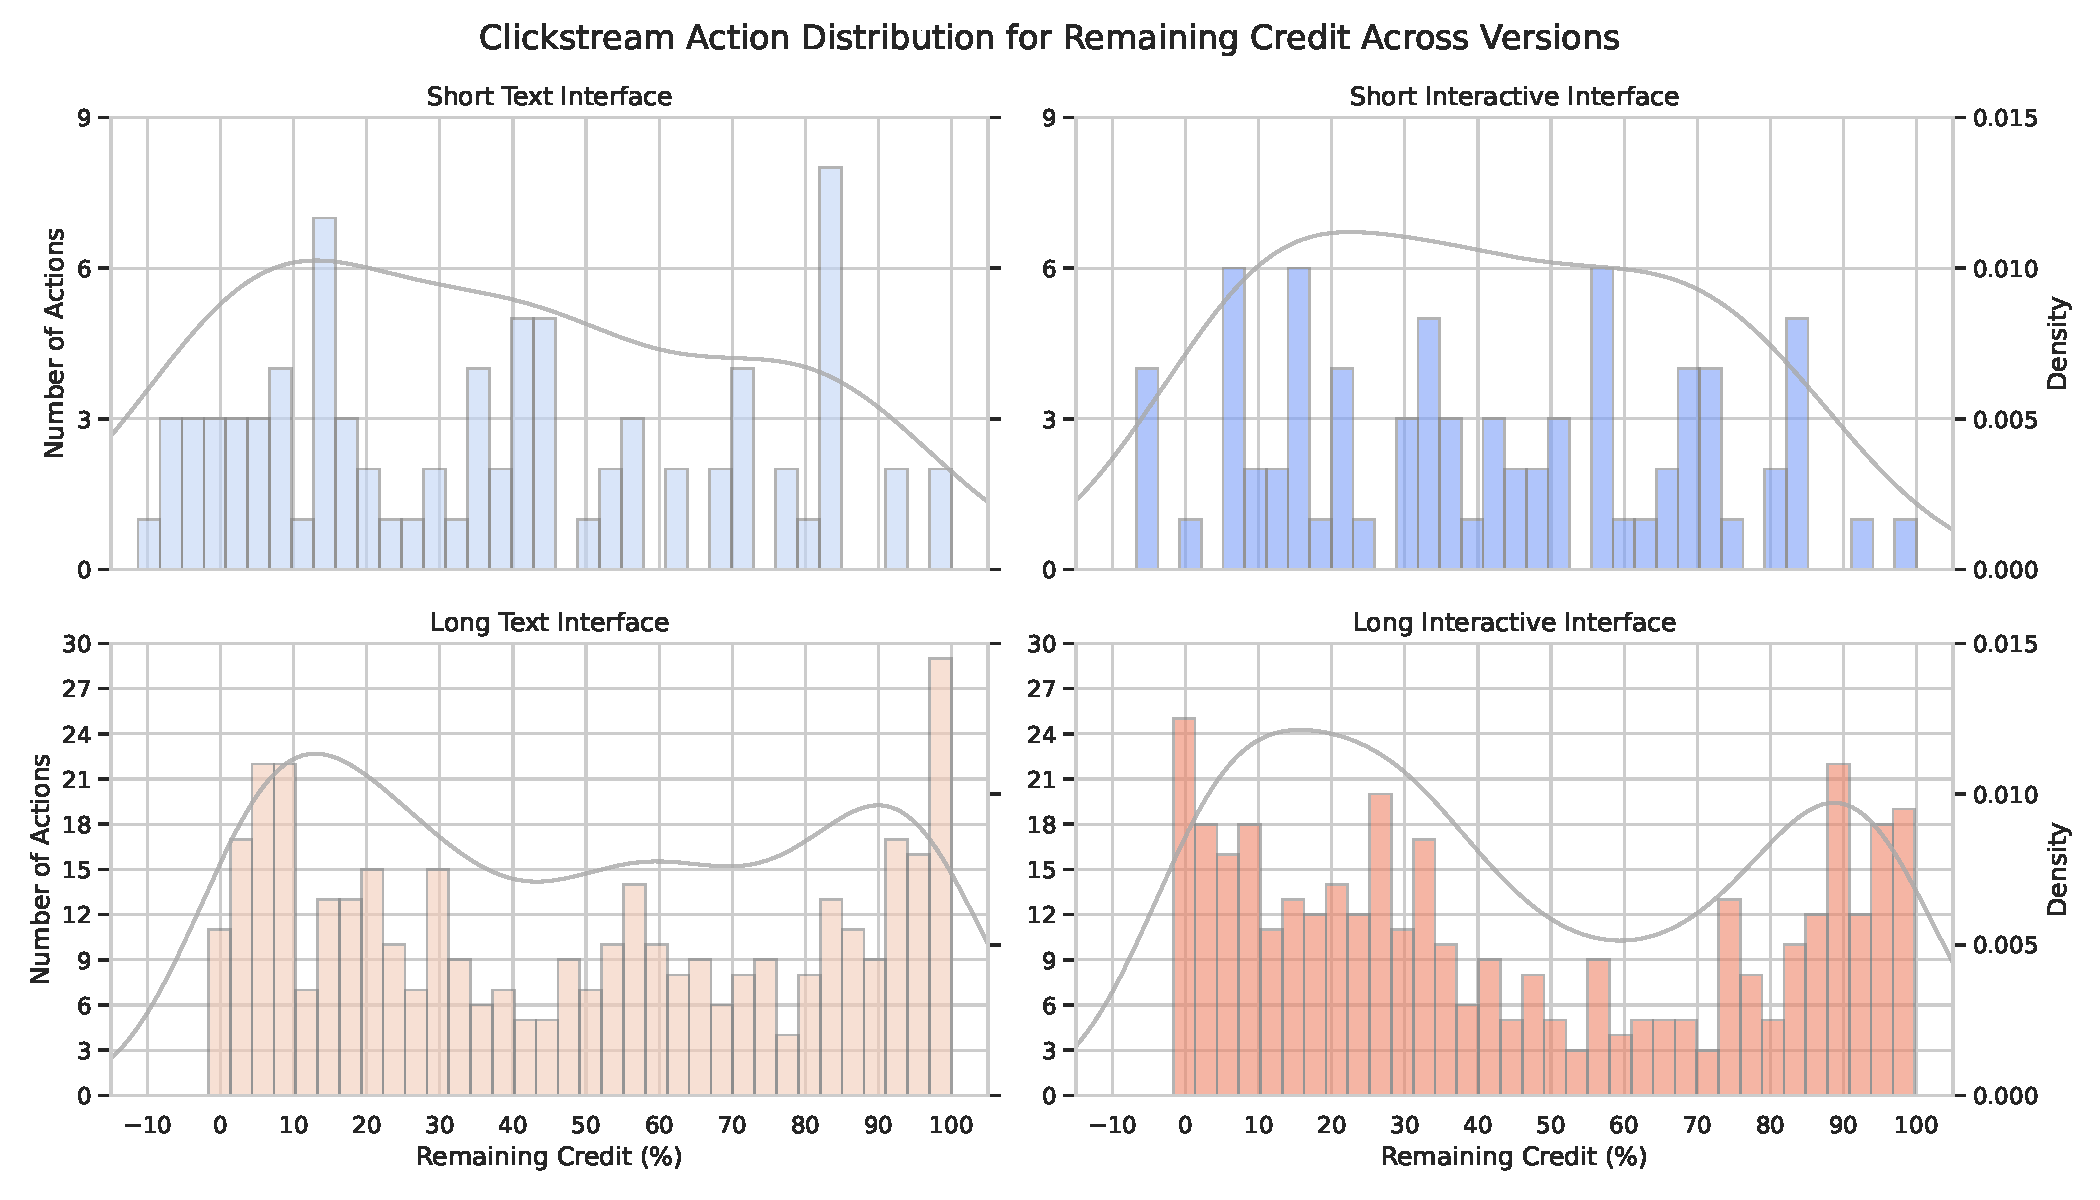
\includegraphics[width=\textwidth]{content/image/results/clickstream_action_distribution.pdf}
    \caption{voting actions across all options (needs to update chart text, remove normalization, and change the dot colors.)}
    \label{fig:voting_all}
\end{figure}

\subsection{Budget and Voting Behaviors}
Next, we examine participants' voting behavior and how it changed throughout the progress. Given that we observe significant differences in voting time changes comparing text interface and interactive interface for the long option survey, we focus on deciphering the voting action changes between these two experiment conditions in this subsection.

Figure~\ref{fig:voting_all} plots the time of voting actions over the remainder of the participant's budget across the text and interactive interface across all four groups. In other words, different from~\textcite{quarfoot2017quadratic} focusing on the number of accumulated votes over an individual's time, where they showed QV voters make more revisions than Likert Surveys, we focused on the budget scarcity which can influence QS respondents' behaviors.

In this plot, we see two distinct patterns between the short survey and the long survey in terms of participant behaviors. Only in the long surveys did participants exhibit more actions when the budget was abundant and when it began to run out, with the long interactive interface being more significant.

\begin{figure}[ht]
    \centering
    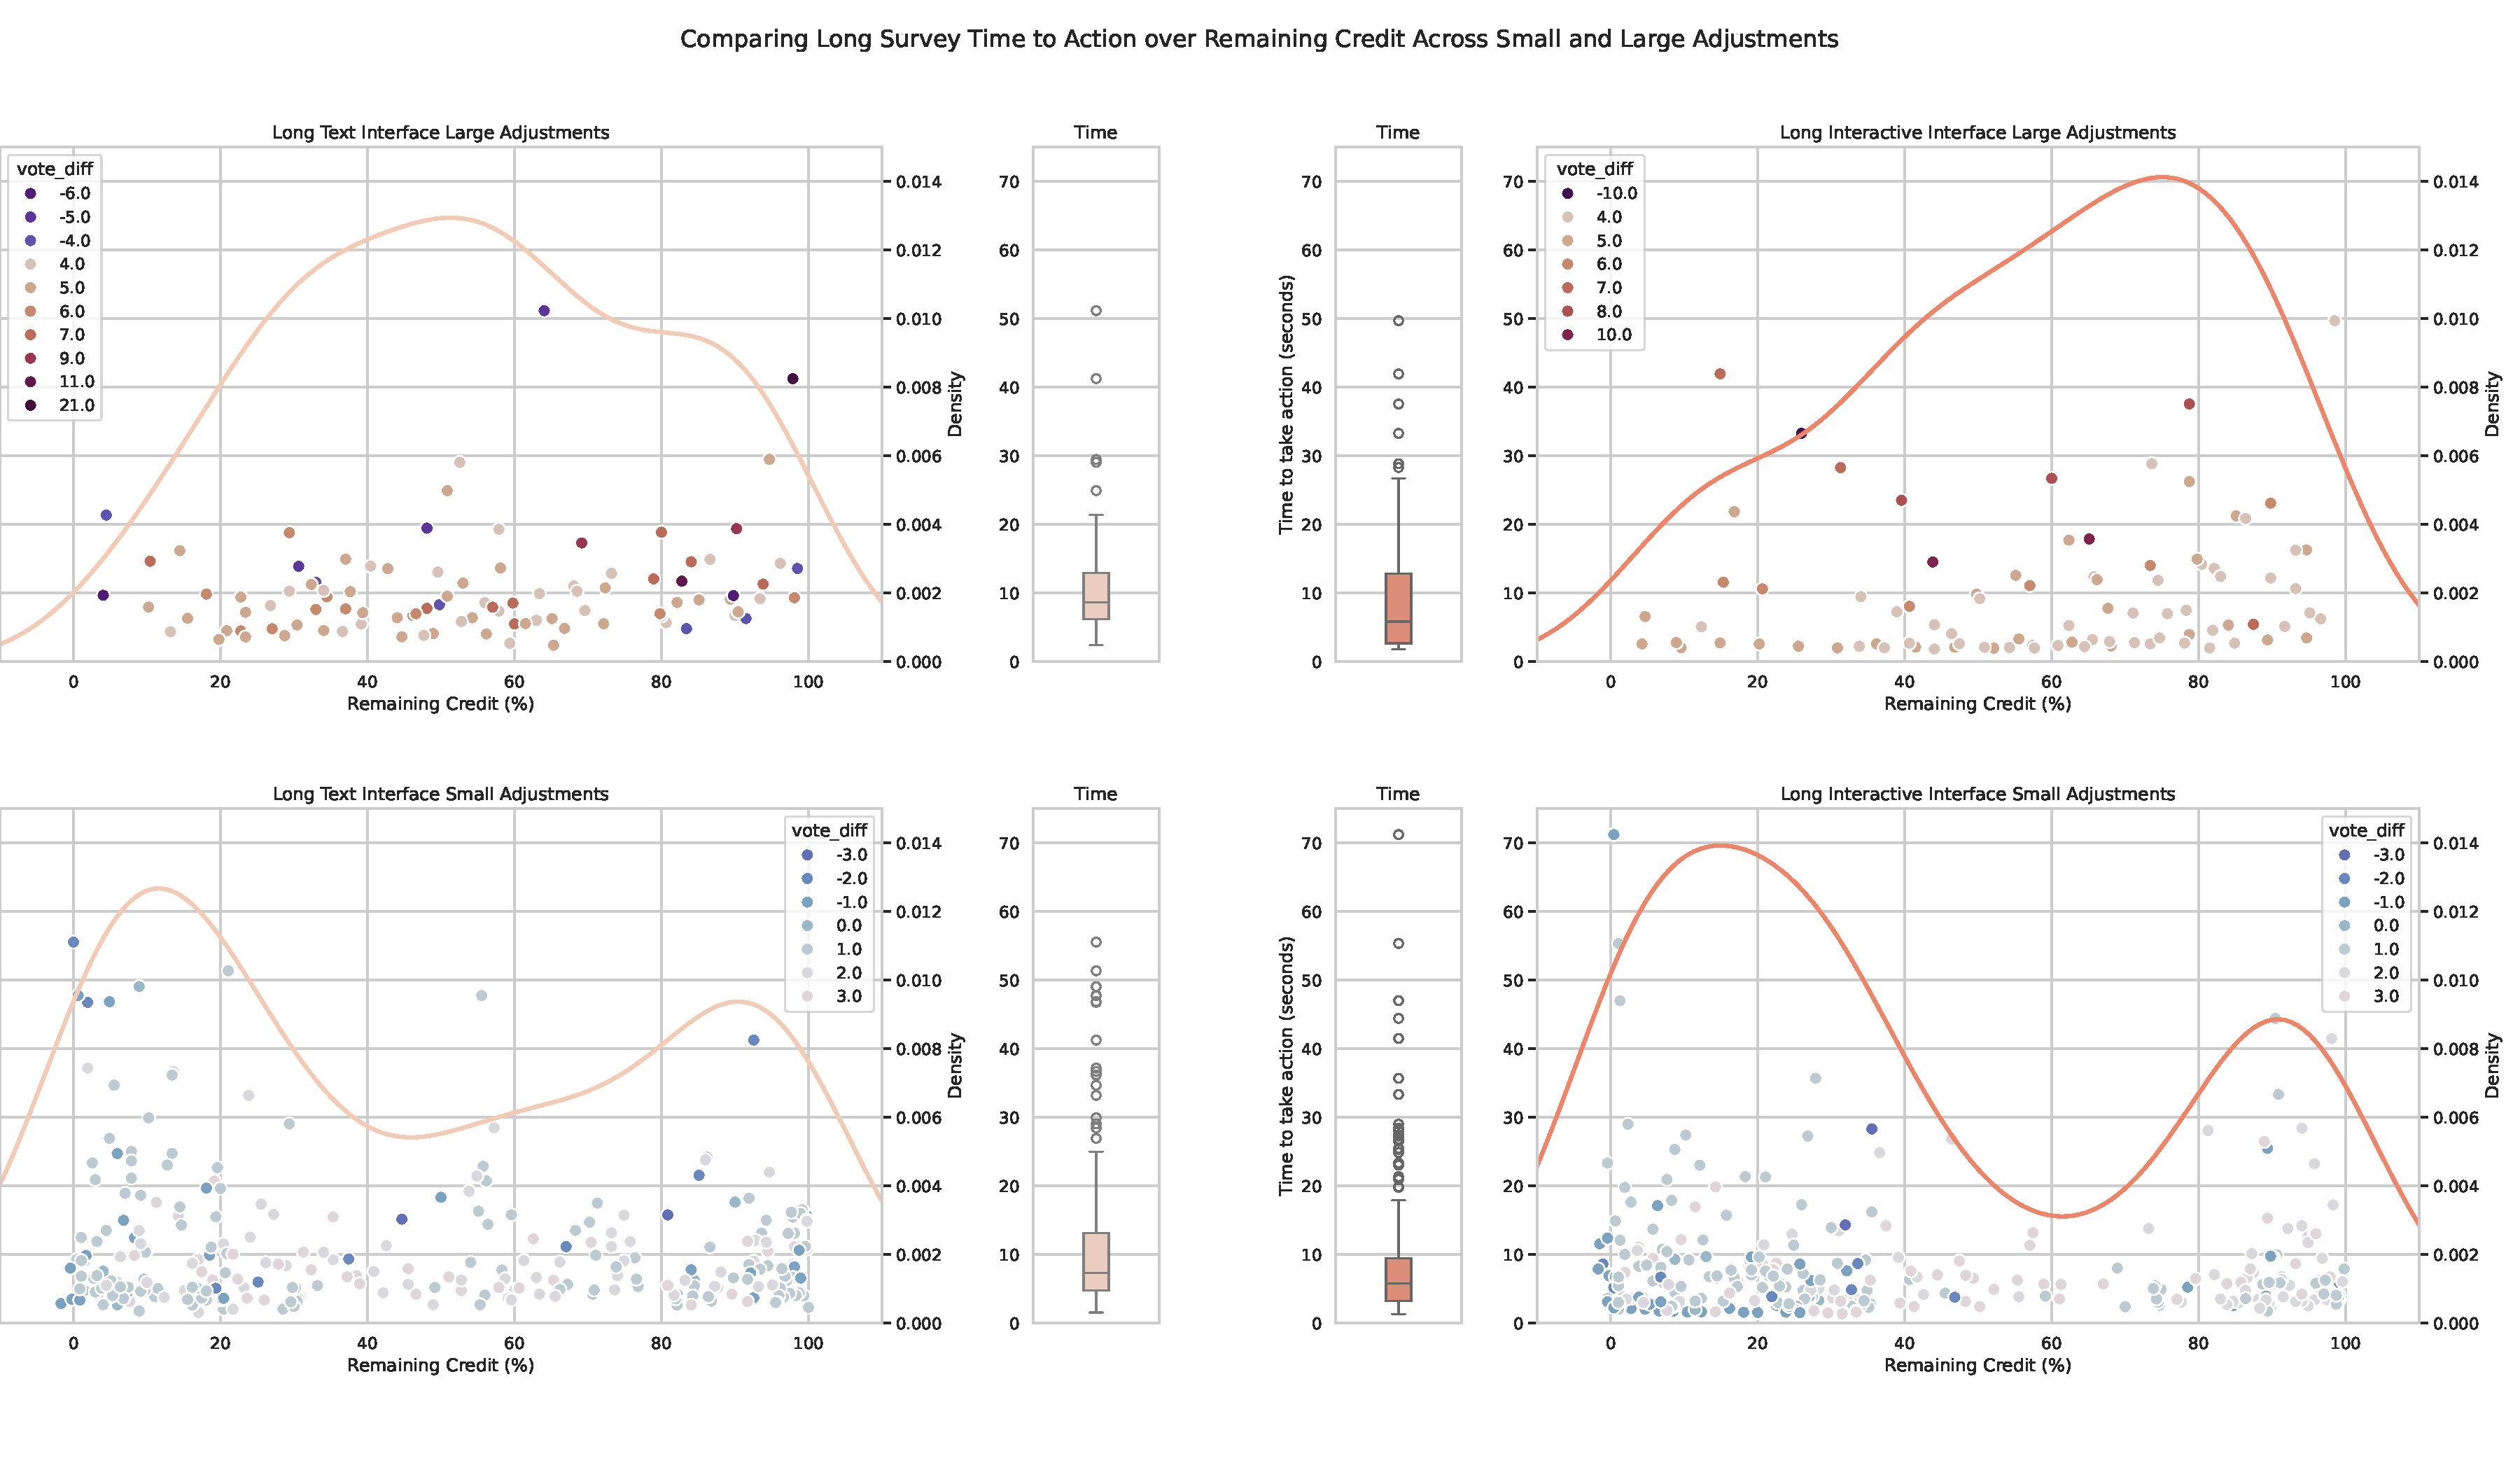
\includegraphics[width=\textwidth]{content/image/results/combined_density_plots.pdf}
    \caption{Breakdown of voting actions (needs to update chart text)}
    \label{fig:voting_v3_v4}
\end{figure}

Thus, we further separated the behaviors where participants made bigger changes or smaller changes to the option, specifically for the long version. In Figure~\ref{fig:voting_v3_v4} , we define an adjustment of four or more votes as a large adjustment which we plotted in the first row of the Figure. Adjustments of three or fewer votes are considered small adjustments.

First, we are able to surface the bimodal action distribution in both plots, with a even stronger signal for long interactive interface participants. Second, the plot demonstrated a clear cluster of voting actions in the bottom left corner of the interactive interface for small vote adjustments. In other words, participants made much smaller but more rapid adjustments when their budgets were running low. Second, larger adjustments are made when the participants have more options comparing the two plots on the first row. We interpret this behavior as participants in the interactive interface have constructed a clearer image of option preferences and, hence, have the ability to take larger strides in allotting their budget and deciding the number of votes at the beginning of the survey. Toward the end, participants using the interactive interface are then making fine-tuned adjustments to ensure that their preferences are reflected in their submissions.

% add qualitative support
\paragraph{Iterative Support from Interactive Interface}
Among all the interviews, when discussing about their experience of the interface, five particpants pointed out the importance of flexibility on the interface and how they took an incremental and iterative approach to navigating their attitude expression. All these participants are using the interactive interface. While this does not mean the study participant using the text interface did not use an iterative approach, but this highlighted the interactive interface encouraged the participants to make iterative and incremental updates. As one participant pointed out:

\begin{displayquote}
I like the fact that it remembers everything that you know. If if you make a mistake, that you don't lose all the work that you've already done. so I think that's very important is that it's an iterative process.

\noindent \hfill -- S019, long interactive interface.
\end{displayquote}

% Ti-Chung Cheng: So what elements of the software interface do you dislike, or like the most, if any, when expressing your preferences on responding to societal issues?
% S009: Hmm! What I like the most actually, probably the sorting function. I think that it really helped me organize my thoughts really, clearly, in terms of what I would dislike the most. really, not that much. I would say. yeah, also, like how we could categorize it, like even within the voting stage rather than just at the categorization stage. 

% Ti-Chung Cheng: Can you tell me a little bit more about the screen? How did the vertical screen help you?
% S037: I think because it helps the layout of, because it's like a long 3 bar. So it's easier for you to to drag and drop, and you can actually sort it, judging by the votes. But I do not do that. But I think this layout is could be helpful in that aspect.

